\chapter{\TitreChapitreCinq}\label{chap:PiegeDipolaire}

\bfig
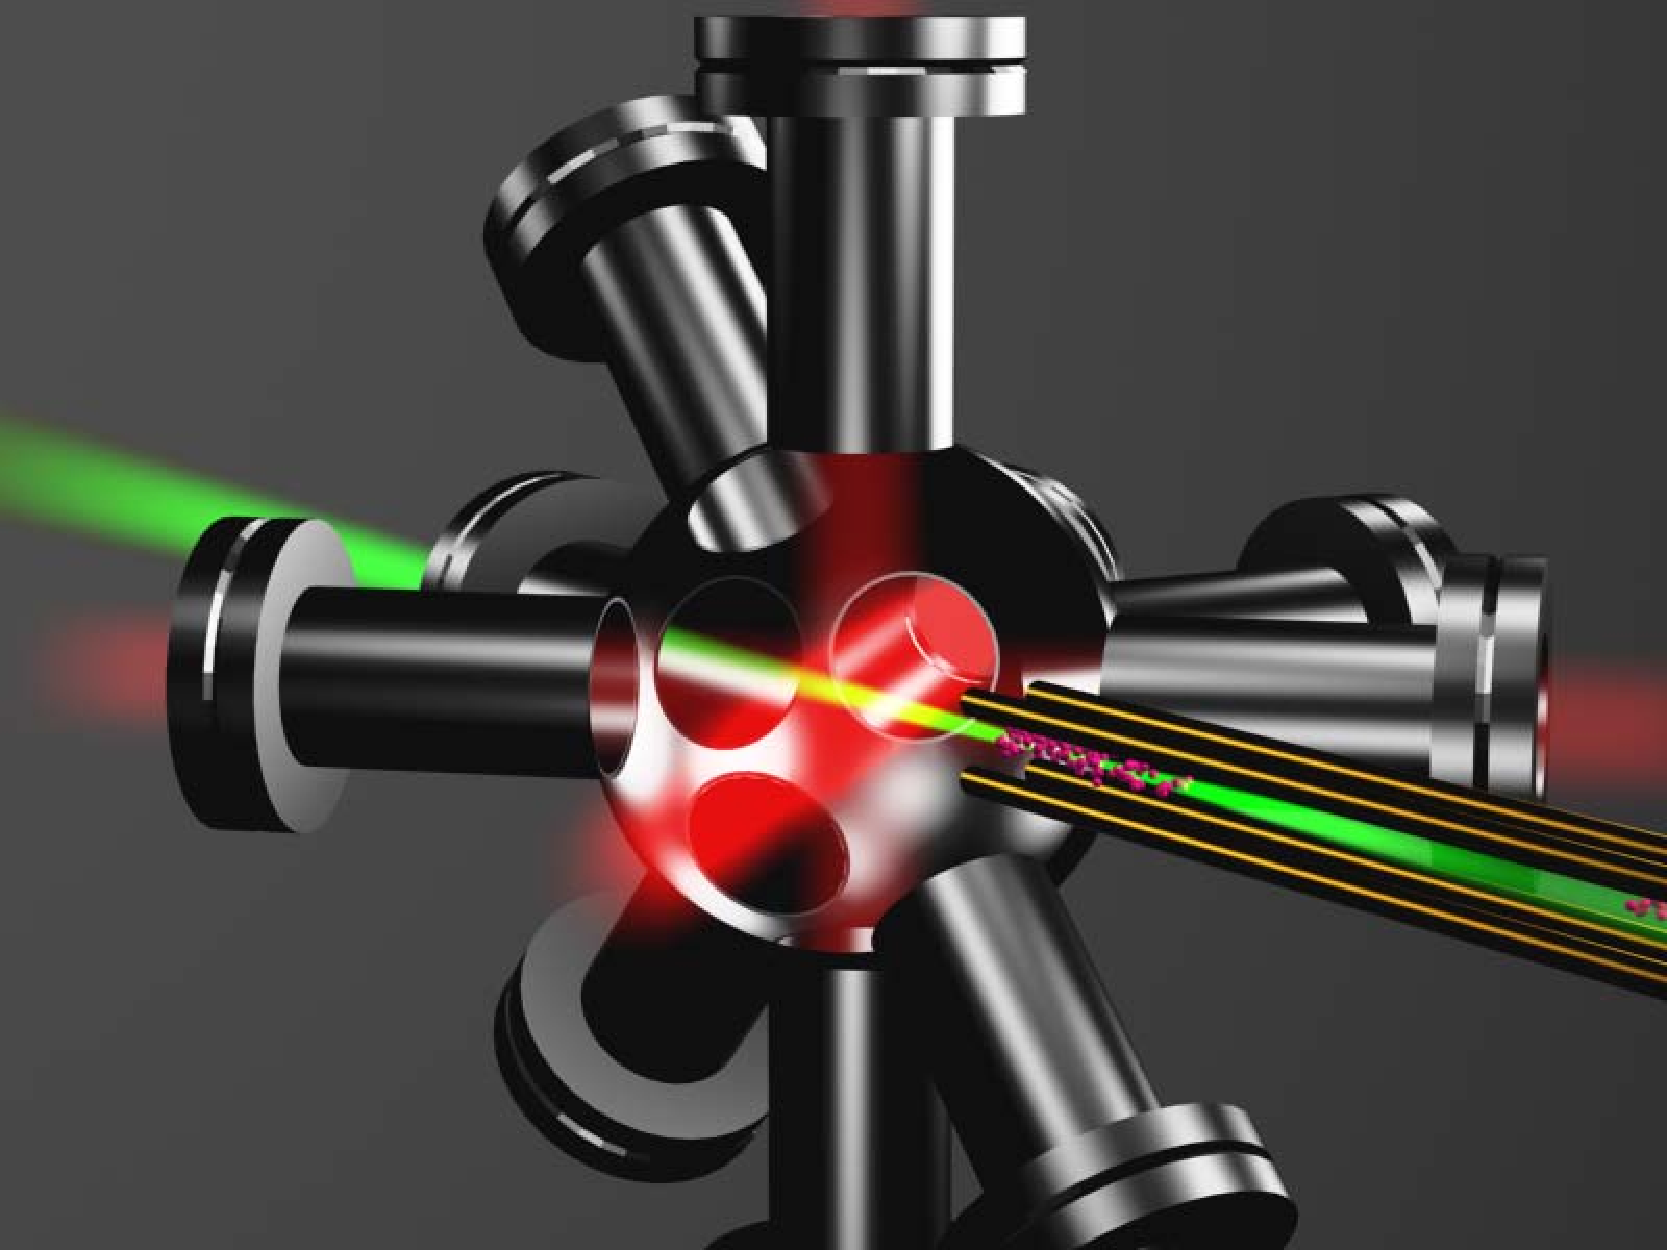
\includegraphics[width=\FigWidth]{P3/ChapitreMonster3ds286}
\SansCaption
\efig

\pagebreak

\minitoc
\vspace{0.5cm}


%13nK = lambda debroglie = 1.5$µ$m ! ! ! ! (à vérifier)
\section{Introduction}

\subsection{De l'amélioration de la préparation des \nats}\label{sec:MotivationPD}

\`A la fin du chapitre~\nref{chap:JetAtomique}, nous avons évoqué trois points soulignant les difficultés liées à l'évaporation d'un \jat. Nous avons conclu qu'il était primordial d'optimiser le nombre de \colels subies en moyenne par chaque atome durant sa propagation dans le \gm. Les chapitres~\nref{chap:Ceramique},~\nref{chap:MiroirMobile} et~\nref{chap:Convoyeur} décrivent trois techniques permettant :
\begin{itemize}
	\item de disposer d'un nouveau moyen d'évaporation dans le \gm (chapitre~\nref{chap:Ceramique}),
	\item de produire un jet plus lent et plus dense (chapitres~\nref{chap:MiroirMobile} et~\nref{chap:Convoyeur}),
	\item d'améliorer les conditions d'évaporation en maintenant momentanément un \pp \td dans le guide (chapitre~\nref{chap:Convoyeur}).
\end{itemize}

\casse

\noindent
Il convient de remarquer que la mise en \oe uvre de ces trois techniques concerne la manipulation d'atomes \ufs, \emph{une fois ceux-ci injectés dans le \gm}.

Rappelons un point que nous avons aussi mentionné dans le chapitre~\nref{chap:JetAtomique} (voir \vpageref{sec:EntreeGuideNonAdiabatique}), quant à l'entrée des \pats dans le \gm : l'extension transverse des \ps (de l'ordre de \mm{1}) entraine un fort échauffement du fait de la soudaine compression dans le \ppt du guide. En pratique, le \p voit sa température décuplée, passant d'environ \microK{50} à quelques \microK{600}.% (voir \vpageref{AN:EntreeGuideEchauffement}).

Il paraît logique de s'intéresser à l'optimisation de cette phase cruciale de l'expérience puisqu'une température initiale du \jat dix fois plus faible pourrait en principe signifier un \tcolel  ainsi qu'une \ddedpup significativement plus élevés. 
\ApplicationNumerique{
En considérant les lois de proportionnalité relatives aux propriétés du \jat (voir \vpageref{RQ:ProportionProprieteJet}), on peut estimer l'influence de la température $T$ du jet.
Ainsi, une température dix fois plus faible conduirait à :
\begin{itemize}
	\item un \tcolel décuplé,
	\item une \ddedpup plus élevée de trois ordre de grandeur.
\end{itemize}
Ces chiffres ne sont bien évidemment qu'une estimation qui ne tient compte que de l'effet de la température $T$, toutes autres choses étant égales par ailleurs (flux $\flux$, vitesse  moyenne $\vmoy$, forme du \pct).
}
Nous avons donc tout intérêt à améliorer le mode de production et d'injection des \pats dans le \gm.



\subsection{Vers l'utilisation d'un \pd}
L'objet de ce chapitre est de présenter une méthode de production de \pats très denses grâce à un piège optique à force dipolaire (aussi appelé \pd , ou encore \termetech{pince optique}). La faible extension transverse des \pats ainsi produits (typiquement \micron{50}) en fait une technique prometteuse quant à l'injection dans un guide.

Nous décrirons la mise en place et la caractérisation d'un laser d'une puissance de \W{300} sur notre \setup. 
Après avoir décrit le protocole de production de \pats denses, nous nous concentrerons sur leur transport par la mise en mouvement du \pd. Un modèle analytique simple nous servira de support pour présenter les résultats expérimentaux liés à l'optimisation du transport.

\casse

\subsubsection{Le piégeage dipolaire de \natufs}
La technique du piégeage d'atomes neutres \ufs par force dipolaire est utilisée depuis 1986~\cite{CBA86}. La mise en \oe uvre du \rpef dans ce type de piège~\cite{ALD95} se prête bien à la production de \becs~\cite{BSC01,CRG03,CRG03a,WHM03,REN04}. En effet, ce type de dispositif présente en général trois avantages par rapport à l'utilisation d'un piège magnétique:
\begin{itemize}
	\item le \pp y est plus confinant et les \dats sont très élevées. L'évaporation y est donc plus rapide (typiquement quelques secondes contre quelques dizaines de secondes pour un piège magnétique%
	\footnote{Nous considérons ici les pièges magnétiques macroscopiques, \cad utilisant des bobines pour générer les \chms. Les expériences de condensation sur puces permettent elles aussi d'évaporer en quelques secondes~\cite{DSI04}.}).
	\item l'absence de bobines pour générer les \chms offre un accès optique optimal.
	\item le piégeage étant purement optique, il est possible d'utiliser un \chm externe pour disposer d'un degré de liberté supplémentaire afin de manipuler les variables internes ou externes des atomes, ou encore pour ajuster les interactions inter-atomiques.
\end{itemize}
%Sur notre \setup, nous 

\subsubsection{Logique de cette approche pour la compression des \pats}
Sur notre \setup, l'utilisation d'un \pd est très intéressante de par les \dats très élevées qu'il est possible d'atteindre par cette technique. 
Si la \dat dans un \pmo de \Rb est typiquement de l'ordre de quelques \atpcc{E10}, elle peut être \val{100} à \val{1000} fois plus élevée dans un \pd~\cite{BSC01}.



\section{Mise en place d'un laser d'une puissance de 300 Watts}

Grâce à un financement spécifique de la \dga, nous avons fait l'acquisition auprès de la société allemande \nomofficiel{IPG} d'un \lyb à fibre d'une puissance de \W{300}. 
Cette section vise à décrire les propriétés de ce laser ainsi que le nouveau \setup que nous avons monté afin d'étudier spécifiquement, et en toute sécurité, la production et la mise en mouvement de \pats très denses.

\subsection{Propriétés du laser}

Le \lyb délivre une puissance laser d'un peu plus de \W{300} à une longueur d'onde $\LO = \nm{1072}$.
Son mode transverse, à la puissance nominale, est très proche%
\footnote{La qualité d'un mode gaussien \temzz est souvent caractérisée par le facteur  $M^2$, appelé \termetech{facteur de qualité}, ou \termetech{facteur de propagation} du faisceau~\cite{SaT91}.}
 d'un mode gaussien \temzz avec un $M^2$ nominal de $\val{1.02}$.
L'onde laser est polarisée linéairement et possède une faible longueur de cohérence longitudinale puisque sa dispersion en longueur d'onde est $\Delta \LO = \nm{2}$. Cette caractéristique ne pose pas de problèmes a priori puisque nous ne souhaitons pas faire interférer ce faisceau avec lui-même%
\footnote{Il en serait tout autrement si nous voulions produire, par exemple, un réseau optique. En effet, une dispersion en longueur d'onde de l'ordre de \nm{1} correspond à une cohérence longitudinale d'environ \mm{1}.}%
. 

\casse

\subsubsection{Mise en sécurité de la salle d'expérimentation}
L'utilisation d'une telle puissance laser dans une salle d'expérimentation implique le respect de certaines règles évidentes de sécurité:
\begin{itemize}
	\item installation d'une cloison isolant l'expérience de celles des autres équipes,
	\item indicateur lumineux indiquant le fonctionnement du laser,
	\item port de lunettes de sécurité,
	\item sécurité coupant instantanément l'émission laser en cas d'ouverture de la porte,
	\item flux d'air filtré sur tout le \setup afin d'éviter les dépôts de poussière sur les composants optiques du \ldp%
	\footnote{Avec une telle puissance, une poussière brulée sur un composant optique pourrait endommager sa surface.
	% Le faisceau serait alors diffusé aléatoirement.
	}.
%	\item éclairage puissant de l'expérience afin d'assurer une bonne contraction de la pupille à tout instant. Ceci vise à minimiser d'éventuel dommage en cas de problème.
\end{itemize}
De plus, il est de rigueur d'utiliser des composants optiques présentant de faibles coefficients de dilatation thermique et disposant d'un traitement de surface adapté. 
\Remarque{
Au delà de la simple nécessité d'éviter les interférences et pertes de puissance laser, il faut garder à l'esprit que chaque pour-cent de la puissance laser correspond à plusieurs watts. Par exemple, chaque face non-traitée d'une lentille ou d'un hublot réfléchira typiquement $\val{4}\%$ de la puissance lumineuse, soit potentielement \W{12}.
}

\subsubsection{Précautions particulières avec les hublots}
Nous attirons l'attention sur le fait que les hublots de l'enceinte à vide doivent être \emph{minutieusement sélectionnés}. En effet, nos hublots, bien qu'adaptés à de telles puissances (en termes de matériaux et de traitement de surface) ont présenté quelques signes inquiétants dès l'utilisation d'intensités de l'ordre de \Wpcmc{1000} à la surface du hublot. Certain points des hublots se mettent alors à émettre une lumière blanche intense (probablement le signe d'une température locale très élevée). Ces points étant apparemment aléatoirement répartis, il est conseillé de faire, pour chaque hublot, des tests préalables avant de construire le dispositif final. Une fois l'enceinte sous \uv, il est en effet difficilement envisageable de changer un hublot défectueux%
\footnote{D'autres équipes de recherches manipulant des \ldps à \micron{1.5} et \micron{10} ont aussi abouti à la même conclusion.}.


\subsection{Montage d'un nouveau \setup}
Comme nous l'avons dit, le but de l'utilisation d'un tel laser est d'augmenter la \dat des \ns dans un \pd, avant que ceux-ci ne soient injectés dans le \gm. Aussi, le faisceau laser de piégeage doit être aligné suivant l'axe $z$ du guide. 
Cependant, l'utilisation de telles puissances laser ne permet pas, à cette étape d'investigation, de \sotosay{simplement} combiner la présence du \lyb et du \gm. En effet, si les lasers habituellement utilisés ont peu d'impact sur les matériaux constituant notre \setup, nous pourrions sérieusement endommager ce dernier avec une puissance de \W{300}.
%Il faut d'ailleurs mentionné que ce type de laser est normalement utilisé dans l'industrie pour la découpe de métaux. 
Si le \fl entrait dans le guide, des réflexions sur les tubes du cuivre et sur la face interne du tube de verre induiraient une diffusion totalement incontrôlable d'une forte puissance lumineuse.

%De plus, les hublots qui permettent l'accès optique à la chambre de \pmo ne sont pas traités pour l'anti-réflection à une \lo de $\LO=\nm{1072}$.  Il est donc préférable d'utiliser des hublots traités.

\casse

Il a ainsi été décidé de procéder à l'étude des possibilités offertes par ce laser en montant un nouveau \setup, plus simple car sans \gm, et possédant des hublots spécifiquement prévus pour l'utilisation d'une grande puissance laser à cette \lo (voir la figure~\nref{fig:ChangeSetup}).
%
\bfighs
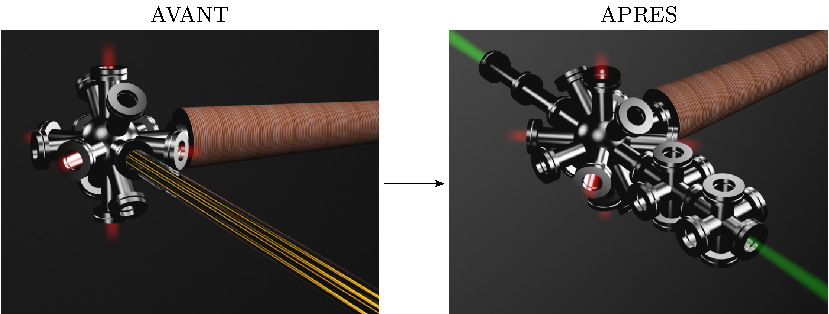
\includegraphics{P3/MonsterChangeSetup}
\CaptionFig{Représentation schématique des deux versions du \setup, avant et après changement. La deuxième version ne fait plus intervenir le \gm. }
\label{fig:ChangeSetup}
\efigh

\subsection{Contrôle de la puissance et de la positon du \fld}
Notre \lyb est conçu pour opérer à sa puissance nominale de \W{300} pour répondre aux caractéristiques spécifiées par le constructeur (en termes de qualité de faisceau, de largeur spectral, de bruit d'intensité, etc\ldots).
Il est possible de n'utiliser qu'un pourcentage de la puissance nominale, mais le boîtier de commande du laser ne permet pas de la faire varier dynamiquement.

Pour pouvoir contrôler dynamiquement la puissance laser utilisée pour produire le \pd depuis le dispositif informatique de l'expérience, nous utilisons un \aom refroidi par eau. La puissance laser diffractée%
\footnote{Nous obtenons, dans les meilleurs conditions, jusqu'à environ \val{85}\% de lumière diffractée dans l'ordre $1$.}
 dans l'ordre $1$ est pilotée, via une tension de commande analogique, par l'alimentation électrique du modulateur. Celle-ci est capable de délivrer jusqu'à \W{35} d'onde \rf dans un câble coaxial. 

\EnFaitNon{
Afin de s'affranchir des inévitables fluctuations de puissances lumineuses, nous avons de plus mis en place une boucle d'asservissement. Le système informatique de notre expérience commande directement cette boucle de manière à avoir une puissance proportionnelle à la tension de commande.

Une autre source de perturbation pour nos expériences réside dans les fluctuations de la position du \fld. Un système d'asservissement opto-mécanique de la position du laser%
\footnote{Ce système d'asservissement a été essentiellement développé par Antoine Couvert, doctorant, et Tomasz Kawalec, post-doctorant.}%
, nous permet d'assurer un positionnement stable. Nous ne détaillons pas ce système ici.
 }
%\bfig
%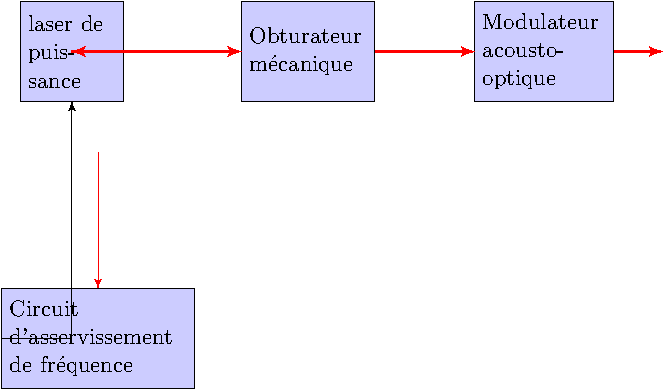
\includegraphics{P3/MonsterAsservissementLaser}
%\CaptionFig{}
%\label{fig:AsservissementLaser}
%\efig




\section{Piégeage optique par \fds}

Lorsqu'un atome est placé dans un champ de lumière laser, il se produit un \termetech{couplage dipolaire électrique} qui résulte de l'interaction du \che $\Evect$ de l'onde avec le \da $\Pvect$ induit par ce-dernier. Il en résulte principalement deux processus qui peuvent influer sur les degrés de liberté externes de l'atome :
\begin{itemizel}
	\item la \emph{force de pression de radiation}, qui provient de cycles d'absorption d'un photon laser, suivi d'une ré-émission spontanée. Cette force joue un rôle important lorsque la pulsation laser est proche d'une résonance d'une transition électronique de l'atome. Notons par ailleurs que son caractère dissipatif la rend peu adaptée pour manipuler des ensembles atomiques dont la température est inférieure à la température de recul ($\Trecul\approx\microK{0.4}$ pour le \Rb).
	\item la \termetech{\fd} qui dérive d'un potentiel et intervient quand l'intensité laser n'est pas uniforme dans l'espace et que sa pulsation est désaccordée par rapport à une transition. La \fd présente l'avantage d'être non-dissipative, ce qui permet de manipuler les atomes de manière cohérente et à des températures arbitrairement faibles.
Pour cela, il faut cependant que l'émission spontanée puisse être négligée (voir la \autoref{sec:PiegeageEtChauffage}). 
\end{itemizel}

Dans l'annexe~\nref{annexe:ForceDipolaire} nous décrivons la \fd électrique. On y trouvera 
%une approche qualitative en utilisant un raisonnement classique, puis 
un traitement quantique menant à une interprétation en terme de déplacement des niveaux d'énergie de l'atome. 

\subsection{Potentiel dipolaire et chauffage pour un atome alcalin}\label{sec:PiegeageEtChauffage}

Dans cette sous-section, nous donnons l'expression du potentiel dipolaire dans le cas d'un atome alcalin. Nous discuterons par la suite du taux de chauffage lié à l'émission spontanée des atomes piégés.


\subsubsection{Potentiel dipolaire}

Dans le cas d'un atome alcalin dans son état fondamental $\OrbitalSJ$, l'expression~\nref{eq:DeltaEiFinalAlcalin} de l'annexe~\nref{annexe:ForceDipolaire} nous donne l'expression du potentiel dipolaire en fonction du moment angulaire total $F$ et du sous-état magnétique $\mF$. Cette expression n'est valide que pour un désaccord du laser grand devant la structure hyperfine %
\nome{\Udip}{Potentiel dipolaire}%
:
\begin{align}
	&\Udip\xyz = \PropUI \times I\xyz 
\virguleformule
\text{ avec }
	\label{eq:UpropI}
\\
	\PropUI &= 
	\frac{\pulsSpont\,{\LO}^3}{16\,\pi^2\,c}\,
	\left[
	\left(\dfrac{1
	}{\desacU}
	+\dfrac{1
	}{\desacU + 2\,\pulsLaser}
	\right)\,
	\left( 1 - \polarindice \, \gF \, \mF \vphantom{\dfrac{1}{\desacU + 2\,\pulsLaser}}
	\right)
	+ 
	\left(\dfrac{1
	}{\desacD}
	+\dfrac{1
	}{\desacD + 2\,\pulsLaser}
	\right)\,
	\left( 2 + \polarindice \, \gF \, \mF \vphantom{\dfrac{1}{\desacU + 2\,\pulsLaser}}
	\right)
	\vphantom{\,\sum_{j \in \OrbitalPJdeux} }
	\right]\nonumber
\virguleformule
\end{align}%
\nomeRemonte{\PropUI}{Facteur de proportionnalité entre $\Udip$ est l'intensité laser}{1.5cm}%
où $\gF$ est le \termetech{facteur de Landé}, $\polarindice$ est un indice qui caractérise la polarisation de l'onde laser ($\polarindice=0,\pm1$ respectivement pour linéaire et circulaire $\sigma^\pm$). Les pulsations $\desacU$ et $\desacD$ correspondent aux désaccords de l'onde laser par rapport aux \termetech{lignes} $D_1$ et $D_2$.
% (voir la figure \vref{fig:RbNiveaux}).

%Ces lignes $D_1$ et $D_2$, dont les \los sont notées $\LO_1$ et $\LO_2$, sont communes à tous les atomes alcalins et correspondent à une transition de type $\OrbitalSJ\rightarrow\OrbitalPJun$ et $\OrbitalSJ\rightarrow\OrbitalPJdeux$.
%
Dans toute la suite, nous considèrerons le piégeage d'atomes de \Rb avec un \fld possédant une polarisation linéaire ($\polarindice=0$).

\ApplicationNumerique{
Évaluons la constante de proportionnalité $\PropUI$ dans le cas du \Rb dans son état fondamental et en considérant l'interaction avec une onde polarisée \emph{linéairement} ($\polarindice=0$) issue de notre \lyb ($\LO=\nm{1072}$) : 
\[
\PropUI \approx \SI{-2.06E-36}{\joule\per({\watt\per\square\meter})}
\pointformule
\]
Afin d'avoir, par exemple, un piège d'une profondeur correspondant à une température $T=\milliK{1}$, il faut donc une intensité d'environ $\Wpcmc{E6}$.
}

\subsubsection{Taux de chauffage}
Comme nous l'avons précisé au début de la section, la \fd est conservative et permet a priori de manipuler des ensembles atomiques à des températures arbitrairement faibles. En pratique, il faut cependant tenir compte de la diffusion de photons qui va se traduire par un taux de chauffage. Dans la limite considérée précédemment, où le désaccord $\desac$ est grand devant la structure hyperfine de l'atome, on peut montrer~\cite{GWO99} que le taux de diffusion par atome $\Gammadif$ est approché%
\footnote{Les termes \termetech{anti-résonants} sont négligés dans cette expression. }
 par l'expression:
\begin{equation}
	\Gammadif 
	\approx I \, \frac{\pulsSpont^2\,{\LO}^3}{16\,\pi^2\,c\,\hbar}
	\, \frac{1}{\deseffcarre}
%	\, \left(\frac{2}{{\desacD}^2} + \frac{1}{{\desacU}^2} \right)
	\pointformule
	\label{eq:TauxAbsorption}
\end{equation}
où nous avons utilisé la notation : $\frac{1}{\deseffcarre} \equiv \left(\frac{2}{{\desacD}^2} + \frac{1}{{\desacU}^2} \right)$.

\noindent On exprime le taux de chauffage $\dT$ par la relation suivante ($\vrecul$ étant la vitesse de recul) :
\begin{equation}
	\dT 
	= \Gammadif \, \frac{m\,\vrecul^2}{\kb} 
	\approx
	I \, \frac{\pulsSpont^2\,\hbar\,\LO}{4\,c\,\kb\,m}
	\, \frac{1}{\deseffcarre}
%	\, \left(\frac{2}{{\desacD}^2} + \frac{1}{{\desacU}^2} \right)
	\pointformule
	\label{eq:TauxChauffage}
\end{equation}
On comprend quel est l'intérêt d'utiliser un laser très désaccordé de manière à minimiser ce taux de chauffage.
\ApplicationNumerique{
Dans nos conditions, et pour le \Rb, nous pouvons exprimer le taux de chauffage $\tdT$ au fond d'un piège de profondeur $\Uprof$. En considérant que $\Uprof$ correspond à une température $T_0=\ttfrac{\Uprof}{\kb}$, on peut écrire :
\begin{equation}
	\dT = T_0 \times \smun{2.4E-3} 
	\pointformule
	\label{eq:ChauffageSurT0}
\end{equation}
Ainsi, pour prendre un exemple, si la profondeur du \pd correspond à \milliK{1}, le taux de chauffage dû à la diffusion sera de $\dT\approx\microKps{2.4}$.
}
Cette application numérique montre que, dans nos conditions, le chauffage sera toujours négligeable par rapport à la profondeur du \pd (pour des temps de piégeage de quelques secondes). Celui-ci est donc parfaitement adapté au \rpef (voir la \autoref{sec:EvapPD}).


\casse


\subsection{Piégeage dans un faisceau unique}

\subsubsection{Faisceau gaussiens \temzz}
Nous supposerons dans toute la suite que le mode transverse de propagation du \fl est un \temzz. Dans la suite, l'origine des cordonnées \xyz sera pris comme étant le point de focalisation du faisceau.
Rappelons l'expression de l'intensité $\Ixyz$ d'une telle onde monochromatique se propageant suivant l'axe $z$~\cite{SaT91}:
\begin{equation}
	\Ixyz = \frac{2\,P}{\pi\,\wz^2}\,\Expo{-\dfrac{2\,(x^2+y^2)}{\wz^2}}
	\virguleformule
	\label{eq:ITEMZZ}
\end{equation}
où $P$ %
\nome{P}{Puissance de \fld}%
est la puissance de \fl. 
Le rayon à $\ttfrac{1}{\rm e^2}$ dépend de la coordonnée $z$ :
\begin{equation}
	\wz = \wzexpr
	\virguleformule
	\label{eq:WZ}
\end{equation}
où $\wzero$ %
\nome{\wzero}{\termetech{Waist} du \fl}%
est le rayon minimum, ou \termetech{waist} du faisceau. 
La \ldr $\zR$ %
\nome{\zR}{Longueur de Rayleigh du \fl}%
s'exprime en fonction du \waist via :
\begin{equation}
	\zR = \zRexpr
	\pointformule
	\label{eq:ZR}
\end{equation}
La figure~\nref{fig:TEMzz} représente un profil typique d'intensité et permet d'illustrer les notations introduites dans les équations~\nref{eq:ITEMZZ} à~\nref{eq:ZR}.
\bfighs
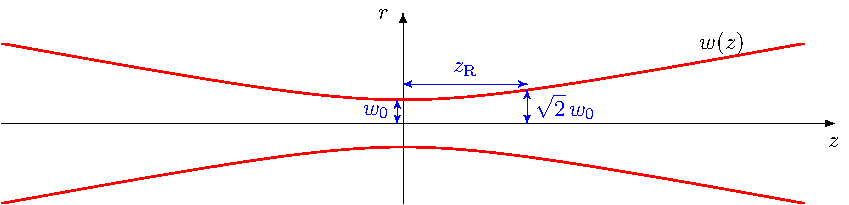
\includegraphics{P3/MonsterTEMzz}
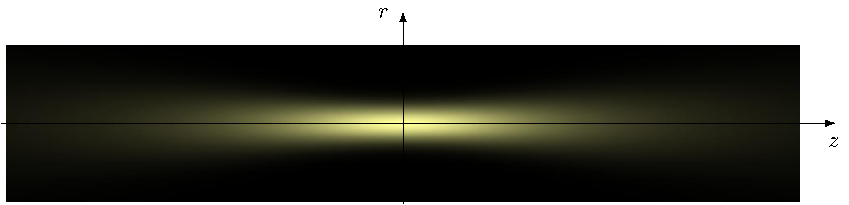
\includegraphics{P3/MonsterTEMzzDensityPlot}
\CaptionFigs{Représentation de la fonction $\wz$ qui donne le rayon à $\ttfrac{1}{\rm e^2}$ du \fl en fonction de la coordonnée $z$. Le graphe inférieur représente en unités arbitraires de couleur l'intensité en fonction des cordonnées ($z,r$). Si on considère un faisceau typique, ayant un \waist de $\wzero=\micron{50}$, ces graphes sont dessinés à l'échelle \val{3} selon $z$ et à l'échelle \val{80} selon $r$. La \ldr $\zR$ est définie par $w(\zR) = \sqrt{2}$.}
\label{fig:TEMzz}
\efigh

\casse

\subsubsection{Potentiel de piégeage}
D'après les équations~\nref{eq:UpropI} et~\nref{eq:ITEMZZ} à~\nref{eq:ZR}, nous pouvons calculer le potentiel $\Udipxyz$ engendré par un faisceau unique du \lyb:
\begin{equation}
	\Udipxyz = - \Uprof\,\left(\frac{\wzero}{\wz}\right)^2\,\Expo{-\dfrac{2\,(x^2+y^2)}{\wz^2}}
	%\mbox{, avec $r$}
	\virguleformule
	\label{eq:UdipxyzFaisceauUnique}
\end{equation}
où $\Uprof$ est la profondeur du \pd (on prend par convention $\Uprof>0$).
%
La figure~\nref{fig:FormesUdipHarmonique} représente le potentiel $\Udip$ suivant l'axe longitudinal $z$ et suivant une direction transverse :
\begin{itemize}
	\item dans chaque plan transverse $\xy$ le potentiel $\Udipxyz$ possède une forme gaussienne de demi-largeur à $\ttfrac{1}{\rm e^2}$ donnée par $\wz$.
	\item suivant l'axe $z$, $\Udip(0,0,z)$ est de forme lorentzienne avec une demi-largeur à mi-hauteur donnée par $\zR$.
\end{itemize}
%
\bfighs
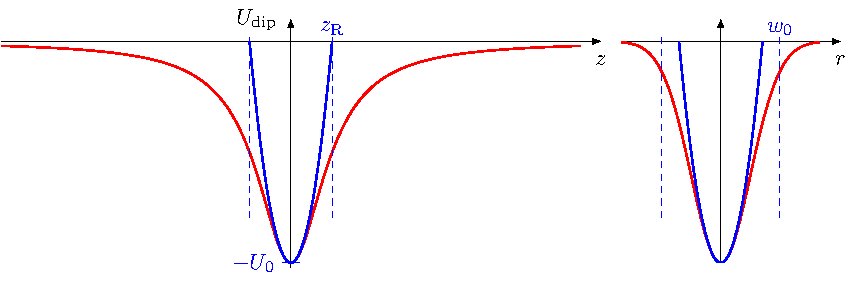
\includegraphics{P3/FormesUdipHarmonique}
\CaptionFigs{Représentation du \ppllor, selon l'axe $z$ du \pd, ainsi que du \pcthar. On représente en plus le \pphar correspondant au développement limité au fond du \pd. Si on considère un \fl dont le \waist vaut $\wzero=\micron{50}$, l'abscisse du graphe de gauche est à l'échelle ($\zR \approx \mm{7}$), alors que celle du graphe de droite est grossie $200$ fois. Ceci illustre le fait que le \pd en faisceau unique est toujours beaucoup plus confinant transversalement.}
\label{fig:FormesUdipHarmonique}
\efigh

\RemarqueTitre{Anisotropie du \pd en faisceau unique\label{Rq:AnisotropiPD}}{
On constate grâce à l'équation~\nref{eq:ZR} que le rapport entre la taille longitudinale $\zR$ du piège et sa taille transverse $\wzero$ est donné par 
\[
\frac{\zR}{\wzero} = \pi\,\frac{\wzero}{\LO}
\virguleformule
\] 
\cad par le rapport entre le \waist $\wzero$ et la \lo $\LO$. On comprend donc que ce type de \pd en faisceau unique soit toujours très anisotrope avec un confinement typiquement \val{10} à \val{100} fois plus fort selon les directions transverses (voir la figure~\nref{fig:FormesUdipHarmonique}).
}

\casse

Dans le cas où un \nat est piégé à l'\eqthdy dans le potentiel $\Uprof$ il est commode d'introduire le paramètre sans dimension $\eta$ %
\nome{\eta}{Paramètre décrivant la profondeur du piège par rapport à la température}%
:
\begin{equation}
	\eta
	 \equiv \dfrac{\Uprof}{\kb\,T}
	 \virguleformule
	\label{eq:EtaPD}
\end{equation}
qui est défini par le rapport des deux énergies en jeu :
\begin{itemize}
	\item la profondeur $\Uprof$ du \pd,
	\item l'énergie thermique moyenne $T$ des atomes du jet.
\end{itemize} 

\subsubsection{Approximation par un piège harmonique}
Si l'énergie thermique $\kb\,T$ des atomes piégés dans le potentiel $\Udipxyz$ est très inférieure à la profondeur $\Uprof$, \cad si $\eta\gg1$, l'extension du \nat suivant l'axe $z$ est faible devant la \ldr $\zR$, et est radialement faible devant le \waist $\wzero$. Dans ce cas les atomes n'explorent qu'une toute petite partie du \pp, et on peut considérer avec une bonne approximation que le piège est harmonique en effectuant le développement limité au deuxième ordre en \xyz:
\begin{equation}
	\Avec{\Udipxyz}{\eta\gg1} \approx ~~ \Udiphxyz ~~ \equiv ~~ \Uprof\,\left( -1+\dfrac{x^2+y^2}{\ttfrac{\wzero^2}{2}}+\dfrac{z^2}{\zR^2} \right)
	\pointformule
	\label{eq:Udiphxyz}
\end{equation}%
\nome{\Udiph}{Approximation harmonique du potentiel dipolaire au fond du piège}%
Les pulsations d'oscillation radiale (dans le plan transverse $\xy$) et longitudinale (selon l'axe $z$) sont données respectivement par:
\begin{equation}
%	\PulsTrans = \sqrt{\frac{4\,\Uprof}{m\,\wzero^2}} 
	\PulsTrans = \frac{1}{\wzero}\,\sqrt{\dfrac{4\,\Uprof}{m}}
	\mbox{~~~~~~et~~~~~~} 
%	\PulsLong = \sqrt{\frac{2\,\Uprof}{m\,\zR^2}}
	\PulsLong = \frac{1}{\zR}\,\sqrt{\dfrac{2\,\Uprof}{m}}
	\pointformule
	\label{eq:FreqUdiphxyz}
\end{equation}
La figure~\nref{fig:FormesUdipHarmonique} représente le \pphar correspondant. 
%\bfigh
%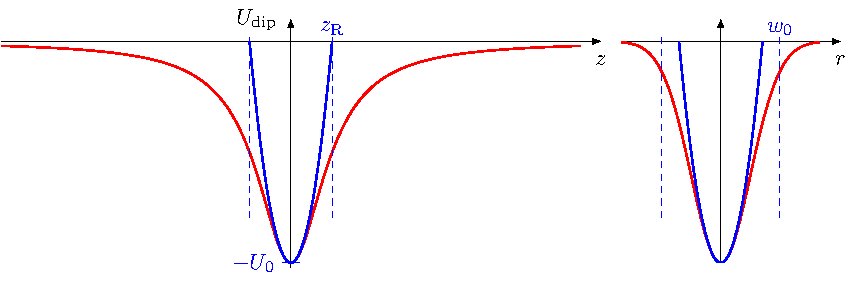
\includegraphics{P3/FormesUdipHarmonique}
%\CaptionFig{Représentation du \ppllor, selon l'axe $z$ du \fl, ainsi que du \pcthar (voir la figure~\nref{fig:FormesUdipxyz}). }
%\label{fig:FormesUdipHarmonique}
%\efigh
Celle-ci montre en outre que ce développement n'est valable que sur une extension longitudinale relativement faible.
\ApplicationNumerique{Pour déterminer la plage sur laquelle l'approximation harmonique $\Udiph(0,0,z)$ est correcte, on peut utiliser la formule 
\[
z_\chi = \frac{\zR}{\sqrt{\chi}}
\virguleformule
\]
qui définit la distance $z$ pour laquelle $\Udiph(0,0,z)$ correspond à $\Udip(0,0,z)$ avec un écart relatif inférieur à $\ttfrac{1}{\chi}$. 
En terme d'énergie, ceci correspond à un paramètre $\eta_\chi\equiv\ttfrac{\Uprof}{\kb\,T}$ tel que:
\[
\eta_\chi = {\chi+1}
\pointformule
\]
Ainsi, l'approximation harmonique $\Udiph$ s'écarte de $\Udip(0,0,z)$ de $\val{10}\%$ pour $z\approx\ttfrac{\zR}{3}$ qui correspond à $\eta\approx\val{11}$. Un atome explorant une telle plage du \pplor voit sa pulsation d'oscillation $\PulsLongLor$ plus élevée de $6\%$ par rapport à la pulsation $\PulsLong$ du piège $\Udiph$.
}
\Remarque{
Il convient de noter que l'approximation harmonique selon les axes transverses est toujours meilleure que selon l'axe longitudinal. On peut facilement obtenir des expressions de $z_\chi$ et $\eta_\chi$ pour le \pc gaussien. Celles-ci font intervenir la fonction \termetech{$W$ de Lambert}%
\footnotemark%
, mais on peut écrire avec une bonne approximation :
\[
r_\chi \approx \frac{\wzero}{\sqrt{\chi}}
\text{~~et~~}
\eta_\chi \approx  \frac{\chi + 1}{2}
\pointformule
\]
\finformule
}
\footnotetext{La fonction \termetech{$W$ de Lambert} est la fonction réciproque de la fonction définie par $f(x)=x\,\expo{x}$.}


\subsection{Lois de proportionnalité et ordres de grandeur}\label{sec:Proportionalite}

Nous avons exprimé quelques grandeurs physiques en fonction de la profondeur $\Uprof$ et des paramètres géométriques ($\wzero$ et $\zR$) du \pd. Nous donnons ici les lois de proportionnalité en fonction de la puissance $P$ du \fl et du \waist $\wzero$. Ces deux paramètres sont en effet ceux sur lesquels nous pouvons agir dynamiquement%
%\footnote{Nous avons en effet utilisé une technique de zoom optique afin de pouvoir modifier le \waist $\wzero$ du \fl (voir la \autoref{sec:ZoomOptique}).}%
.
Nous exprimerons aussi les caractéristiques importantes d'un \nat piégé et supposé à l'\eqthdy dans le \pphar $\Udiph$, en fonction de sa température $T$. 

\newcommand{\fois}{\times}
\newcommand{\with}{~~,&\text{avec ~~ }}
\newcommand{\foiswith}[3]{\alpha_{#1} \times #2%\fois &&\!\!\!\!\!\!\!\!#1 %
\with &&{\alpha_{#1}=#3}&\approx }
\Resultat{
D'après les équations~\nref{eq:UpropI},~\nref{eq:ITEMZZ},~\nref{eq:ZR} et~\nref{eq:FreqUdiphxyz}, nous exprimons les caractéristiques du \pd :
\begin{subequations}
\begin{align}
	\Uprof &= \foiswith{1}{\frac{P}{\wzero^2}
	}{
	\frac{2\,\PropUI}{\pi} }
	\SI{1.31E-36}{SI}%
	\\
	\PulsTrans &= \foiswith{2}{\frac{\sqrt{P}}{\wzero^2} 
	}{
	\sqrt{\frac{8\,\PropUI}{\pi\,m}} }
	\SI{6.03E-6}{SI}%
	\\
	\PulsLong &= \foiswith{3}{\frac{\sqrt{P}}{\wzero^3}
	}{
	\sqrt{\frac{4\,\PropUI\,\LO^2}{\pi^3\,m}} }
	\SI{1.46E-12}{SI}%
%	\\
%	\dT &= \foiswith{1}{\frac{\sqrt{P}}{\wzero^3}
%	}{
%	\sqrt{\frac{4\,\PropUI\,\LO^2}{\pi^3\,m}} }
%	\SI{1.46E-12}{SI}%
\end{align}	
\label{eq:LoisProportionnalitePiege}
\end{subequations}
\finformule
}
Si nous considérons un \n composé de $N$ atomes piégés dans un état proche de l'\eqthdy (défini par la température $T$), nous pouvons de plus exprimer les paramètres importants tels que la \dat moyenne $\overline{\dens}$, la \dmdedpup $\overline{\rho}$ et le \tcolel moyen par atome $\overline{\gammacol}$:%
\nome{\overline{\dens}}{Densité atomique moyenne du \n dans le \pd}%
\nome{\overline{\rho}}{Densité moyenne dans l'\edp du \n dans le \pd}%
\nome{\overline{\gammacol}}{Taux de \colels moyen du \n  dans le \pd}

%\renewcommand{\foiswith}[1]{\fois &&\!\!\!\!#1 \with &&{#1}&\approx }
\Resultat{
\finformule
\begin{subequations}
\begin{align}
	\overline{\dens} &= \foiswith{4}{\frac{N\,P^\frac{3}{2}}{\wzero^7\,T^\frac{3}{2}}
	}{
	\frac{4\,\PropUI^\frac{3}{2}\,\sqrt{2}\,\LO}{{\kb}^\frac{3}{2}\,\pi^{4}} }
	\SI{3.59E-27}{SI}%
	\\
	\overline{\rho} &= \foiswith{5}{\frac{N\,P^{\frac{3}{2}}}{\wzero^7\,T^3}
	}{
	\frac{16\,\PropUI^\frac{3}{2}\LO\,\hbar^{3}}{\kb^3\,\pi^\frac{5}{2}\,m^\frac{3}{2}} }
	\SI{2.36E-56}{SI} \label{eq:LoisProportionnaliteNatRho}%
	\\
	\overline{\gammacol} &= \foiswith{6}{\frac{N\,P^{\frac{3}{2}}}{\wzero^7\,T}
	}{
	\frac{8\,\PropUI^{\frac{3}{2}}\,\LO\,\sigma}{\pi^\frac{9}{2}\,\sqrt{m}\,\kb} }
	\SI{1.99E-41}{SI}%
\end{align}	
\label{eq:LoisProportionnaliteNat}
\end{subequations}
\finformule
}

\ApplicationNumerique{
Exprimons quelques profondeurs de piège $\Uprof$ et pulsations d'oscillation $\PulsTrans$ et $\PulsLong$ pour différent \waists $\wzero$ et différentes puissances $P$ :
\newcommand{\Ueg}{{{\Uprof}}=}
\newcommand{\Puz}{\PulsTrans=}
\newcommand{\Pur}{\PulsLong=}
\begin{footnotesize}
\begin{center}
	\begin{tabular}{|*{5}{c|}}
	\hline
	\backslashbox{$\wzero$}{$P$}
	&\W{1}&\W{10}&\W{100}&\W{300}\\
	\hline
&$\Ueg\microK{2.1}$&$\Ueg\microK{21}$&$\Ueg\microK{210}$&$\Ueg\microK{620}$\\
	\micron{200}	
&$\Puz\rps{140}$&$\Puz\rps{440}$&$\Puz\rps{1400}$&$\Puz\rps{2400}$\\
&$\Pur\rps{0.17}$&$\Pur\rps{0.54}$&$\Pur\rps{1.7}$&$\Pur\rps{2.9}$\\
	\hline
&$\Ueg\microK{8.2}$&$\Ueg\microK{82}$&$\Ueg\microK{820}$&$\Ueg\microK{2500}$\\
	\micron{100}
&$\Puz\rps{560}$&$\Puz\rps{1800}$&$\Puz\rps{5600}$&$\Puz\rps{9700}$\\
&$\Pur\rps{1.35}$&$\Pur\rps{4.3}$&$\Pur\rps{13.5}$&$\Pur\rps{23.5}$\\
	\hline
&$\Ueg\microK{33}$&$\Ueg\microK{330}$&$\Ueg\microK{3300}$&$\Ueg\microK{9900}$\\
	\micron{50}
&$\Puz\rps{2200}$&$\Puz\rps{7100}$&$\Puz\rps{22000}$&$\Puz\rps{39000}$\\
&$\Pur\rps{11}$&$\Pur\rps{34}$&$\Pur\rps{110}$&$\Pur\rps{190}$\\
	\hline	
	\end{tabular}
\end{center}
\end{footnotesize}
}

\subsubsection{Anharmonicité du \pplor}
Si le \nat occupe une large extension spatiale du \pplor, on ne peut plus définir une pulsation $\PulsLong$ d'oscillation puisque celle-ci dépend de l'amplitude du mouvement. En revanche, on peut calculer la pulsation $\PulsLongLor(\zmaxTraj)$ pour chaque trajectoire atomique en fonction de l'abscisse maximale $\zmaxTraj$ de sa trajectoire sur l'axe $z$ du \pd. L'expression exacte fait intervenir une fonction \termetech{elliptique de type E}, mais peut être approchée numériquement par une loi quadratique%
 \footnote{L'expression exacte est : $
	\PulsLongLor(\zmaxTraj) = \PulsLong \, \left(
	\frac {2}{\pi }
	\,\sqrt{1+{\left(\frac{\zmaxTraj}{\zR}\right)}^{2}}
	\,{\it EllipticE}\left( i\,\frac{\zmaxTraj}{\zR} \right)
	\right)^{-1}
%	\label{eq:PulsLongLorElliptic}
$%
. L'expression approchée~\nref{eq:PulsLongLor} s'écarte de moins de $3\%$ de la valeur exacte sur une plage d'amplitude allant jusqu'à $\zmaxTraj= 5 \, \zR$.} :
\begin{equation}
	\PulsLongLor(\zmaxTraj) \approx \frac{\PulsLong}{1+ \val{0.67}\, \left( \dfrac{\zmaxTraj}{\zR} \right)^2}
	\pointformule
	\label{eq:PulsLongLor}
\end{equation}

%\subsubsection{Influence de la gravité}
% EXPRESSION DE LA LONGEUR EFFECTIVE DU PIEGE, DE LA PUISSANCE CRITIQUE, ...


\subsection{Caractérisation expérimentale du \pd}
\subsubsection{Caractéristiques géométriques}
Les caractéristiques géométriques du \fl sont très importantes dans la mesure où ce sont elles qui déterminent la profondeur, la taille et les fréquences d'oscillation dans le \pd. Il est donc primordial de disposer d'une mesure expérimentale de ces caractéristiques. Il va de soi que la puissance élevée du \lyb pose quelques problèmes de compatibilité avec les instruments de mesures usuels.

La solution retenue consiste à effectuer un diagnostic sur la lumière non-réfléchie par miroir. Nos miroirs sont en effet traités pour optimiser la réflexion du \ldp (avec un coefficient de réflexion $R=\val{99.6}\%$), et sont par ailleur faits d'un bloc de verre transparent aux faces parallèles. Nous pouvons ainsi utiliser un très faible pourcentage de la lumière laser afin de l'envoyer sur un capteur CCD. 

\casse

\noindent
La figure~\nref{fig:DignosticLaser} illustre le montage et une mesure de profil d'intensité.
\bfighs
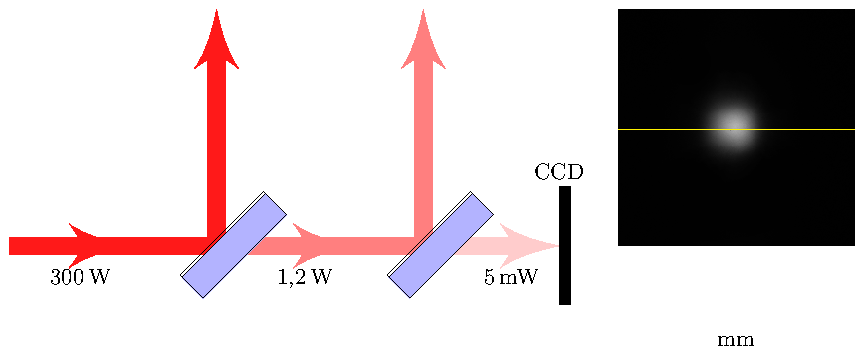
\includegraphics{P3/MonsterDignosticLaser}
\CaptionFigssss{Le \fl est réfléchi sur l'un des miroir de notre \setup. Environ \val{0.4}\% de la lumière traverse un miroir muni d'un traitement anti-reflet. En utilisant cette \sotosay{fuite} de lumière, et en recommençant une seconde fois cette opération sur un autre miroir, on récupère une fraction d'environ \val{E-5} de la puissance du faisceau initial. Un capteur CCD dont on peut régler précisement l'exposition peut alors être utilisé pour mesurer la répartition d'intensité (image sur la droite). Le graphe représente en unité arbitraire le profil d'intensité le long de la ligne horizontale sur l'image. La ligne pointillée (rouge) qui y est superposée  correspond à l'ajustement d'une fonction gaussienne sur le profil.}
\label{fig:DignosticLaser}
\efigh
En effectuant ce type de mesure en plusieurs points de l'axe du \fl, nous avons constaté la présence d'aberrations sphériques. 
%On observe par exemple une asymétrie du faisceau, avec 

\Remarque{
 Ces aberrations géométriques sont partiellement dues à la qualité des composants optiques (nous n'utilisons que des lentilles sphériques). Nous avons aussi constaté une dépendance de ces aberrations vis à vis de la puissance délivrée par le boîtier du \lyb. Le faisceau est de bonne qualité quand on utilise le laser à sa puissance nominale de \W{300}.

De plus, malgré le flux laminaire d'air filtré sur le \setup, les composants optiques accumulent une fine couche de poussière à l'endroit précis du passage du \fl. Celle-ci détériore fortement la qualité du faisceau. Un nettoyage régulier des composants est donc indispensable.
}

\subsubsection{Mesure des pulsations d'oscillation propres}
Comme nous venons de le mentionner, le \fld possède des aberrations au point de focalisation. Ceci implique que les caractéristiques géométriques propres aux faisceaux gaussiens ne permettent pas de décrire quantitativement le \pd.
Afin d'exploiter au mieux les données expérimentales liées au piégeage de \nat dans le \pd, nous mesurons donc expérimentalement les pulsations propres d'oscillation dans le \pd. Nous procédons différemment pour les pulsations d'oscillation transverse et longitudinale.

\subsubsection{Mesures des pulsations d'oscillation transverse}
Les oscillations dans le plan transverse $\xy$ ont une pulsation typique de l'ordre du kilo hertz. Pour la mesurer, nous utilisons une technique de \termetech{chauffage paramétrique}~\cite{Jau01}. Celle-ci consiste à moduler très légèrement %
\footnote{L'amplitude de modulation correspond à quelques pour-cent de la puissance laser totale.}
 la puissance du \fld à une pulsation donnée, et à observer l'effet sur le \nat qui y est piégé. Quand la pulsation de cette excitation correspond à un multiple pair de la pulsation propre d'oscillation dans le \pd, on observe une forte augmentation de la température du \n. Celle-ci s'accompagne d'une baisse du nombre d'atomes piégés du fait de la profondeur finie du \pd.

 

\subsubsection{Mesures de la pulsation d'oscillation longitudinale}
Les oscillation suivant l'axe longitudinal $z$ ont une pulsation typique de l'ordre de la dizaine de hertz et se prêtent mal à l'utilisation de la technique décrite ci-dessus. Pour mesurer cette pulsation, nous déplaçons rapidement la position du \pd suivant l'axe $z$, d'une distance petite devant la \ldr (la mise en mouvement du \pd est traitée dans la \autoref{sec:MisEnMouvementPD}). Nous observons alors les oscillations du \cdm du nuage.


\section{Production de \nats très denses}
Dans cette section, nous décrivons le protocole expérimental que nous utilisons pour alimenter le \pd en atomes, ainsi que pour y effectuer le \rpef.
Pour les expériences dont il est question dans ce chapitre, le \waist du \fld est mesuré à $\wzero\approx\micron{45}$, ce qui correspond à une \ldr de $\zR\approx\mm{6}$. 

\subsection{Alimentation du \pd}\label{sec:ChargementPD}

L'alimentation du \pd se fait à partir d'un \pmobd%
\footnote{Il s'agit du même \pmo dont les caractéristiques sont données dans le chapitre~\nref{chap:JetAtomique}. Le caractère \bd du piège est obtenu grâce à une configuration ne faisant pas intervenir de champ de confinement longitudinal.}%
.
Bien que n'ayant que peu étudié le chargement du \pd, nos observations sont compatibles avec celles qui font l'objet de la référence~\cite{ATS05}, à savoir que le nombre d'atomes piégés dépend du volume de capture, \cad du volume de recouvrement du \fl avec le \pmo.
Il est en revanche insensible à la puissance du \ldp, à partir d'un certain niveau.
%	

\noindent Nous observons de plus que le nombre d'atomes capturés est très sensible au bon alignement du \flp sur l'axe du \pmo. 
Afin de favoriser le chargement d'atomes dans l'état fondamental $\EtatSF{1}$, la lumière du laser \termetech{repompeur} est occultée sur la zone de recouvrement du \fld et du \pmo. Nous produisons ainsi une configuration de \termetech{\pmo sombre}~\cite{KDJ93}. 


\casse


\subsubsection{Séquence de chargement}
Nous procédons de la manière suivante, le \fld étant présent en permanence, à une puissance $P_0=\W{80}$, ce qui correspond à une profondeur de piège $\Uprof\approx\kb\times\milliK{3}$ :
\begin{itemize}
	\item le \pmobd est chargé pendant \ms{500} à partir du \fat provenant du \ZS (voir la \autoref{sec:PaquetsPmo}). 
	\item le désaccord des faisceaux du \pmo passe alors de $\desac=-\val{3}\,\pulsSpont$ à $\desac=-\val{7.7}\,\pulsSpont$ en \ms{5} (rappelons que $\pulsSpont$ est la largeur naturelle de la transition optique).
	\item les \chms sont coupés, ainsi que le laser repompeur pour obtenir une accumulation des atomes dans le sous-état $\EtatSF{1}$. Cette phase dure typiquement \ms{1}. Les atomes qui ne sont pas capturés dans le \pd sont alors en chute libre.
\end{itemize}
%
Le nombre d'atomes capturés est mesuré en effectuant une image par absorption (voir le chapitre~\nref{chap:Imagerie}). La température est mesurée par la technique habituelle de \termetech{\tof}.
Il est cependant nécessaire d'attendre environ \ms{50} avant d'effectuer des mesures fiables, le temps que les atomes non-piégés du \pmo tombent hors de la zone de mesure.
\Resultat{
Dans ces conditions (\ms{50} après avoir coupé le \pmo), nous obtenons un nombre d'atomes de $N=\val{3E7}$ atomes à une température typique $T\approx\microK{500}$. D'après%
\footnotemark
 les équations~\nref{eq:LoisProportionnaliteNat}, on peut estimer les grandeurs physiques suivantes :
 \begin{itemize}
	\item la \dat, $\overline{\dens}\approx\atpcc{7E12}$,
	\item le \tcolel, $\overline{\gammacol}\approx\smun{800}$,
	\item la \dmdedpup, $\overline{\rho}\approx\val{E-6}$.
\end{itemize}

}
\footnotetext{Les équations~\nref{eq:LoisProportionnalitePiege} et~\nref{eq:LoisProportionnaliteNat} sont valables dans le cas d'un \pphar. Nous les considérons valables ici dans la mesure où la température du \nat correspond à un paramètre $\eta$ d'environ~6.}
%
Étant donné le \tcolel relativement élevé, on peut estimer que, durant les \ms{50} suivant l'extinction du \pmo, une partie des atomes capturés dans le \pd ont déjà été évaporés.

\ifthenelse{\FormatEUE > 0}{}
{\AjouteLigne}

\subsection{Pertes atomiques}
Une donnée importante concernant le piégeage optique dans le \fld est la durée de vie du \nat qui y est piégé. Nous avons mesuré, pour différentes configurations, le nombre d'atomes dans le piège, en fonction du temps de piégeage.
\inlinefig{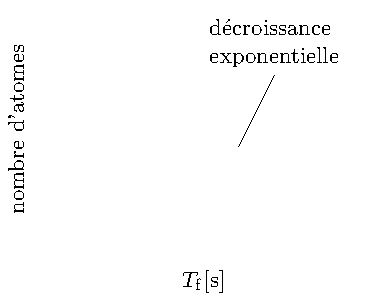
\includegraphics[scale=0.9]{P3/MonsterDureeVie}~} 
Les courbes obtenues sont toutes de la forme de celle représentée ci-contre. Sur ce graphe dont l'échelle des ordonnées est en unités logarithmiques, on distingue deux comportements asymptotiques: 
%\begin{itemize}
%	\item 
	quand le nombres d'atome est assez faible, la décroissance est exponentielle et traduit les pertes d'atomes dues aux collisions avec le gaz résiduel de l'enceinte à vide.
%	\item 
En revanche, pour les grands nombres d'atomes, les pertes sont plus élevées.
%\end{itemize}
\noindent
Nous ne détaillons pas ici les données expérimentales. 
\picskip{0}

\casse

\noindent
Nous nous contentons de préciser que celles-ci sont compatibles avec une loi de décroissance du nombre $N$ d'atomes du type:
\begin{equation}
	\Derive{N}{t} = - \frac{N}{\tau} - \beta\,N\,\overline{\dens}
\virguleformule
	\label{eq:PertesAtomiques}
\end{equation}
où $\ttfrac{1}{\tau}$ est le taux caractéristique de décroissance exponentielle dû aux collisions avec le gaz résiduel et $\overline{\dens}$ est la \dat moyenne dans le \pd. Le coefficient $\beta$ dépendent de l'intensité laser moyenne $\overline{I}$ dans le piège : 
\[
\beta(\overline{I}) \propto \overline{I}^2
\pointformule
\]
Le deuxième terme de la loi~\nref{eq:PertesAtomiques} décrit un processus de perte atomique \termetech{à deux corps} et \termetech{assisté par deux photons}. Les pertes atomiques observées ne sont donc pas dues à un processus de photo-ionisation direct. En effet celle-ci requiert une énergie d'environ \eV{4}, ce qui correspond à plus de trois photons laser. Les pertes sont probablement dues à des processus de photo-associations d'atomes de \Rb. 
Le détail des résultats relatifs à ces expériences seront présentés dans la thèse d'Antoine Couvert.



\subsection{Évaporation et compression de \nats}\label{sec:EvapPD}

Comme nous l'avons souligné dans l'introduction de ce chapitre, l'objectif principal de nos travaux est de développer une technique d'injection de \patufs dans un \gm. Or, juste après la capture dans le \pd, la température du \nat est relativement élevée ($\approx \microK{500}$).
%De plus, nous verrons dans la \autoref{sec:TransportOptimal} que le tr
%Dans cette sous-section nous 

Il est possible d'agir sur les caractéristiques du \n en faisant varier la puissance lumineuse $P$ du \fld en fonction du temps. D'après les expressions~\nref{eq:LoisProportionnalitePiege}, cette opération agit sur deux caractéristiques du piège:
\begin{itemize}
	\item la profondeur $\Uprof$ varie proportionnellement à $P$,
	\item les pulsations d'oscillation $\PulsTrans$ et $\PulsLong$ varient proportionnellement à $\sqrt{P}$.
\end{itemize}

\subsubsection{Refroidissement par \evap}
Nous avons mis en \oe uvre la technique du \rpef consistant à réduire progressivement la puissance lumineuse $P$.
%
Lors d'un processus d'\evap, on peut habituellement considérer que le paramètre $\eta\equiv\ttfrac{\Uprof}{\kb\,T}$ reste approximativement constant. 
La température du \n est alors proportionnelle à la puissance $P$ du \fld :
\begin{equation}
	\begin{cases}
	T\propto P\\
	\eta \approx \const
	\end{cases}
	\text{, durant l'évaporation}
\pointformule
	\label{eq:PropTEtaEvap}
\end{equation}
On pourra consulter avec intérêt la référence~\cite{OGG01} pour obtenir les lois de variation du nombre d'atomes et de la \ddedpup du \n piégé dans le \fld.
%
\Resultat{\label{Res:NuageEvap}
Donnons un exemple typique de \n obtenu après avoir effectué une rampe d'évaporation.
Après la phase de chargement du \pd (se référer à la \autoref{sec:ChargementPD}), nous diminuons la puissance de $P_0\approx\W{80}$ à $P'=\W{0.47}$ en~\seconde{3.3}. 

Durant cette évaporation, le nombre d'atomes diminue de $N\approx\val{3E7}$ à $N'\approx\val{6E6}$, et leur température de $T\approx\microK{500}$ à $T'\approx\microK{3.7}$. La loi~\nref{eq:PropTEtaEvap} sur la température est approximativement vérifiée.
Aussi, on déduit les variations de la \dat, du \tcolel et de la \ddedp:
\[
\begin{cases}
	 \overline{\dens}\approx\atpcc{7E12} &\longrightarrow \overline{\dens}'\approx\atpcc{E12} \\
	 \overline{\gammacol}\approx\val{800} &\longrightarrow \overline{\gammacol}'\approx\val{10}\\
	 \overline{\rho}\approx\val{E-6} &\longrightarrow \overline{\rho}'\approx\val{E-3}
\end{cases}
\]
\finformule
}

\Remarque{
Nous ne somme pas parvenus à produire de \bec dans le \pd en faisceau unique. 
En revanche, nous avons adopté une configuration de faisceaux croisés~\cite{BSC01,KWW05}.
Le faisceau horizontal est croisé à $\SI{45}{\degree}$ par un faisceau ayant un \waist de  \micron{200}. %Leurs puissances respectives sont diminuées pendant l'évaporation qui nous. 
Ce dispositif nous permet de produire un \bec contenant typiquement \val{2E5} atomes en environ \seconde{4}. 
Les travaux effectués avec le \becc seront détaillés dans le manuscrit de thèse d'Antoine Couvert.
}
%Tomek 1234:
%X\cite{CRG03}
%X\cite{BSC01}
%X\cite{KWW05}
%\cite{DJG06}
%Cornelussen 40 41 42 43:
%X\cite{BSC01}
%X\cite{CRG03}
%NOT\cite{CKO03}
%X\cite{REN04}
%Cornelussen 66 69:
%X\cite{CRG03a}
%X\cite{WHM03}
%71 72 73 74 75:
%X\cite{ALD95}
%\cite{KCM00}
%\cite{SMC98}
%\cite{THK03}
%\cite{FSW98}
%Grimm:
%\cite{GWO99}

\subsubsection{Compression du \n}
Il est possible d'augmenter le paramètre $\eta$ en augmentant progressivement la puissance lumineuse $P$. Lors d'une telle compression, on considère que le nombre $N$ d'atomes et la \dmdedpup $\overline{\rho}$ restent constants. D'après l'expression~\nref{eq:LoisProportionnaliteNatRho}, la température du \nat varie alors proportionnellement à $\sqrt{P}$.
La profondeur $\Uprof$ variant proportionnellement à $P$, on en déduit que:
\begin{equation}
\begin{cases}
T \propto \sqrt{P}\\
\eta \propto \sqrt{P}
\end{cases}
\text{, durant une compression à nombre d'atomes constant}
\pointformule
	\label{eq:PropTEtaCompression}
\end{equation}
%D'après les équations~\nref{eq:LoisProportionnaliteNat}, 
\Resultat{
Pour poursuivre l'exemple donné \vpageref[ci-dessus]{Res:NuageEvap}, nous donnons les caractéristiques du \n après recompression. Celle-ci consiste à ré-augmenter la puissance par un facteur $90$, jusqu'à $P''=\W{42}$.
La température passe alors de $T'\approx\microK{3.7}$ à $T''\approx\microK{43}$ et le paramètre $\eta$ atteint $\approx50$. La loi~\nref{eq:PropTEtaCompression} est approximativement vérifiée.
Aussi :
\begin{equation}
	\begin{cases}
	\overline{\dens}'\approx\atpcc{E12} &\longrightarrow 	\overline{\dens}''\approx\atpcc{3E13} \\
	 \overline{\gammacol}'\approx\val{10} &\longrightarrow \overline{\gammacol}'\approx\val{80}\\
	\overline{\rho}''\approx\val{E-3} &\longrightarrow \overline{\rho}''\approx\val{0.6E-3}
	\end{cases}
	\label{eq:NuageRecomp}
\end{equation}
\finformule
}

\casse

\subsection{Retour sur l'injection par une technique de mélasse mouvante}
Pour conclure cette section nous rappelons l'idée qui a motivé la mise en \oe uvre d'un \pd. L'objectif principal est de pouvoir injecter des \patufs et denses dans un \gm (voir la \autoref{sec:MotivationPD}). Nous avons montré dans cette section, que notre \fld permet de produire de tels \ns. 

Nous allons montrer ici que, pour la mise en mouvement de ces \pats, un problème ce pose quant à l'utilisation de la technique de \termetech{mélasse mouvante}~\cite{CSG91} que nous utilisions auparavant pour injecter les atomes issus du \pmo dans le guide (voir le chapitre~\nref{chap:JetAtomique}).
En effet, celle-ci consiste à utiliser la pression de radiation par l'interaction avec des \fls proches de résonance et n'est efficace que si le \n est optiquement peu épais, \cad que l'onde doit pouvoir le traverser sans être significativement absorbée.
%
\RemarqueTitre{Épaisseur optique du \n}{
%Intéressons nous à la \pro du \n dont les caractéristiques sont énoncées ci-dessus. 
La \pro $\OptProf$ est une grandeur qui sera définie et discutée plus en détails dans le chapitre~\nref{chap:Imagerie} (voir \vpageref{eq:DefOptProf}). Elle caractérise l'absorption d'une onde lumineuse traversant le \n.
}
Pour les \ns dont nous avons donné les caractéristiques \vpageref[ci-dessus]{eq:NuageRecomp}, les \pros peuvent typiquement atteindre $\OptProf\approx\val{1E4}$ selon l'axe du \fld et $\OptProf\approx\val{100}$ selon une direction transverse. De telles \pros sont incompatibles avec la technique de \termetech{mélasse mouvante}, et il est nécessaire de disposer d'une autre méthode de mise en mouvement des \nats denses.

Précisément, dans les deux sections suivantes (\nref{sec:TransportOptimal} et~\nref{sec:ModelisationTransport}), nous allons détailler la mise en mouvement du \n grâce à un déplacement au \pd.

{\AjouteLigne}

\section{Transport optimisé de \nats}\label{sec:TransportOptimal}
%
Dans cette section, nous allons détailler l'aspect pratique de la mise en mouvement du \pd. Précisons que, lors d'un déplacement du \fld, les atomes qui y sont piégés vont être excités. La figure~\nref{fig:PiegeBougeAB} illustre ce propos.
%
\bfighs
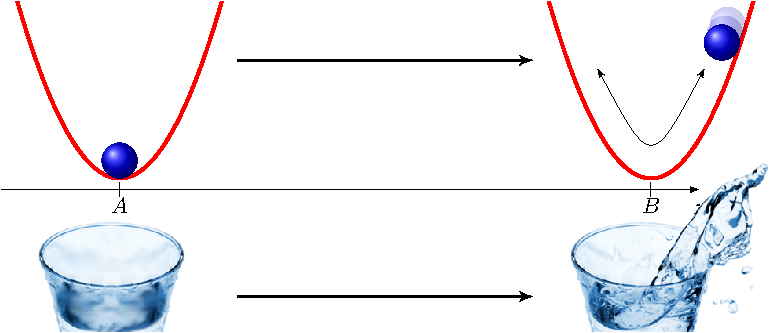
\includegraphics{P3/PiegeBougeAB}
\CaptionFigs{Mise en mouvement d'un piège d'un point $A$ à un point $B$. Une particule initialement au repos au fond du piège peut être excitée suivant son mode d'oscillation dipolaire lors du mouvement. On peut comparer cet effet à celui provoqué par un mouvement brusque d'un récipient contenant un liquide.}
\label{fig:PiegeBougeAB}
\efigh

\noindent 
Nous allons donc être amené à considérer l'excitation d'un \nat, consécutivement à un déplacement du piège.
%Dans cette section et la suivante, nous allons détailler l'étude que nous avons menée quant au transport rapide d'un ensemble atomique. 


\subsection{Mise en perspective et enjeux}
Comme nous l'avons vu en introduction du chapitre~\nref{chap:Convoyeur} (voir \vpageref{sec:ConvIntro}), le transport d'ensembles atomiques \ufs a déjà été mis en \oe uvre dans de nombreux groupes. Rappelons que le transport magnétique sur des distances macroscopiques est principalement effectué en déplaçant mécaniquement des bobines~\cite{LHW03,NSH05}, ou en faisant varier alternativement les courants parcourant un enchevêtrement de bobines~\cite{GBH01}. Nous avons présenté dans le chapitre~\nref{chap:Convoyeur} une nouvelle méthode consistant à déplacer un train d'aimants permanents le long d'un \gm~\cite{LRW06}. 
Le transport dans un \pd se fait soit, en déplaçant mécaniquement un composant optique~\cite{GCL02}, soit en générant un réseau optique \ud dont la position est ajustée en contrôlant le désaccord relatif entre les fréquences de deux \fls contrapropageants~\cite{KAS01,STW06}.
Il est important de remarquer que toutes ces expériences de transport sont effectuées dans le \termetech{régime adiabatique}, \cad que la durée du transport est toujours grande devant la période d'oscillation du piège%
%\footnote{Dans le cas d'un piège est anisotrope, c'est de la période d'oscillation du piège, \emph{suivant la direction du transport}.}%
. 
En effet, une mise en mouvement trop rapide induirait une excitation du mode d'oscillation dipolaire dans le piège (une oscillation du \cdm du nuage). Ceci conduirait donc à un échauffement de l'ensemble atomique, voire à la perte d'une partie des atomes. 

\Resultat{
Nous nous intéressons plus particulièrement à la possibilité de mettre un piège en mouvement sur des échelles de l'ordre de la période d'oscillation, tout en assurant que le \nat n'est pas ou peu excité en fin de transport. 
}
%Nous décrirons le dispositif nous permettant de déplacer le \pd, et, après avoir décrit un modèle analytique unidimensionnel simple, nous interprèterons nos données expérimentales.

\nnRemarque{
On peut se représenté une image naïve de cet effet en imaginant un verre d'eau qu'il faudrait déplacer d'un bout à l'autre d'une table. Si la mise en mouvement du verre est suffisamment lente, on pourra déplacer le verre sans renverser d'eau. Si le mouvement est brusque en revanche, une partie de l'eau sortira du verre.
}

\ifthenelse{\FormatEUE > 0}{}
{\AjouteLigne\AjouteLigne}


\subsection{Mise en mouvement du \pd}\label{sec:MisEnMouvementPD}
La mise en mouvement du \pd est assurée par une unité de translation qui permet de déplacer la lentille de focalisation (voir la figure~\nref{fig:TranslationStage}). Le modèle XMS100 de la société \nomofficiel{Newport} permet de déplacer cette lentille sur une plage de \cm{10}, avec une répétabilité de l'ordre de la centaine de nanomètres.
%
\bfighs
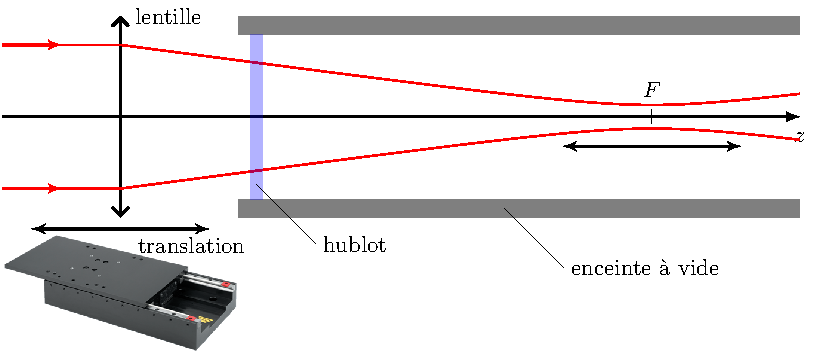
\includegraphics{P3/MonsterTranslationStage}
\CaptionFigs{Le \fl arrive approximativement parallèle sur la lentille. Celle-ci est fixée sur une unité de translation. Le fait de déplacer la lentille selon l'axe optique $z$ permet de déplacer le point de focalisation de la même valeur sans modifier le \waist. }
\label{fig:TranslationStage}
\efigh

\casse

\RetireLigne
\RetireLigne
\RetireLigne
\RetireLigne
\RetireLigne
\RetireLigne

Grâce à ce système nous pouvons imposer un mouvement au \pd le long de l'axe $z$. La position du piège en fonction du temps sera notée $\zct$%
\nome{\zct}{Position, en fonction du temps, du fond du \pd selon l'axe $z$}%
, et nous désignerons sa vitesse instantanée par $\dzct$ %
\nome{\dzct}{Vitesse, en fonction du temps, du fond du \pd selon l'axe $z$}%
et son accélération par $\ddzct$%
\nome{\ddzct}{Accélération, en fonction du temps, du fond du \pd selon l'axe $z$}%
.
Dans toute la suite, nous décrirons ce type de mouvement par un \emph{\pacc}, \cad par la donnée pour chaque instant $t$ de l'accélération imposée au piège. 

De plus, afin de simplifier la description du problème, nous supposerons que :
\begin{itemize}
	\item à l'instant initial $t=0$, le piège est immobile en $z=0$,
	\item la mise en mouvement se fait en un temps fini $\tfin$%
	\nome{\tfin}{Durée de la mise en mouvement}%
	, \cad que l'accélération $\ddzct$ possède un support compact.
\end{itemize}
Ces conditions sont résumées ci-dessous par:
\begin{equation}
\begin{cases}
	\zc_{(t\leqslant0)}   ~~ = ~~  0& \\
	\dzc_{(t\leqslant0)}  ~~ = ~~  0& \\
	\ddzc_{(t<0)} ~~ = ~~ \ddzc_{(t>\tfin)} ~~ = ~~ 0&
\end{cases}
%	\pointformule
	\label{eq:ZcDzcIni}
\end{equation}

La figure~\nref{fig:ProfilDeplacement} représente un exemple particulièrement simple de \pacc correspondant à deux phases d'accélération constante%
\nome{\AccZc}{Valeur maximale de l'accélération du \pd}%
, $\AccZc$ et $-\AccZc$.
Le mouvement durant un temps total $\tfin$, le piège se déplace de $\DistZc=\AccZc\,\ttfrac{\tfin^2}{4}$.%
\nome{\DistZc}{Longueur du déplacement du \pd}%
%
\bfighs
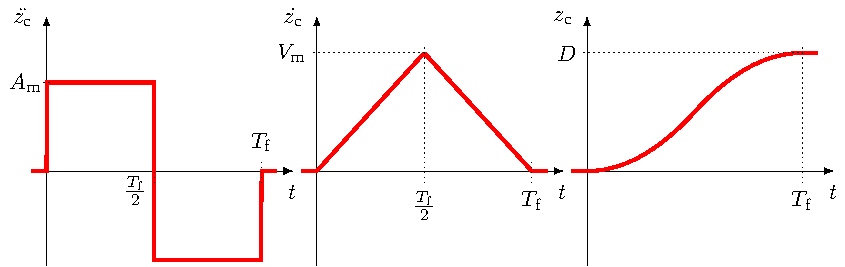
\includegraphics{P3/MonsterProfilDeplacement}
\CaptionFigs{Représentation d'un \pacc particulièrement simple composé de deux phases d'accélération uniforme ($\AccZc$ et $-\AccZc$) de durées égales $\ttfrac{\tfin}{2}$. Les vitesses~$\dzc$ et les positions~$\zc$ correspondantes sont aussi représentées en fonction du temps $t$. Le mouvement durant un temps total $\tfin$, le piège se déplace de $\DistZc=\AccZc\,\ttfrac{\tfin^2}{4}$.}
\label{fig:ProfilDeplacement}
\efigh


\casse

\RetireLigne
\RetireLigne

\subsection{Mesures d'oscillations résiduelles après transport}
Dans cette sous-section nous présentons les données expérimentales liées au transport d'un \n piégé dans le \fld.
Pour deux configurations expérimentales différentes, nous avons mesuré l'amplitude $\Aosc$ %
\nome{\Aosc}{Amplitude des oscillations résiduelles en fin de transport}%
 des oscillations du \cdm du \n à la suite d'une mise en mouvement du \pd.
 
 
\subsubsection{Préparation des \nats}

Pour confronter nos données expérimentales au modèle décrit dans la \autoref{sec:ModelisationTransport}, nous souhaitons nous placer dans des conditions où le \pd peut être considéré comme étant harmonique. Ceci revient à produire un \nat dont le paramètre $\eta\equiv\ttfrac{\Uprof}{\kb\,T}$ est grand.
\`A cette fin, le protocole expérimental utilisé est le suivant:
\begin{itemize}
	\item typiquement \val{3E7} atomes sont chargés dans le \pd (le \waist est $\wzero=\micron{45}$, et la puissance laser est $P_0=\W{80}$). La température est typiquement $T\approx\microK{500}$, et $\eta\approx6$ (voir la \autoref{sec:ChargementPD}).
	\item la puissance $P$ du \ldp est baissée linéairement en fonction du temps jusqu'à une valeur $\Pmin$, induisant ainsi le \rpef du \n.
	\item la puissance est alors ré-augmentée jusqu'à une valeur $\Ptrans$ avant de commencer le transport. Cette phase de re-compression permet d'ajuster la valeur de $\eta$ (voir la \autoref{sec:EvapPD}).
\end{itemize}
La dernière phase (re-compression) est nécessaire à deux égards : ($i$) elle permet d'augmenter la profondeur du piège afin de minimiser les pertes atomiques pendant les phases d'accélération, et ($ii$) elle augmente les fréquences d'oscillation du piège afin de pouvoir effectuer une mise en mouvement rapide.

\vspace{5pt}
\noindent En pratique, nous avons étudié deux configurations que nous dénoterons par :
\begin{ditemize}
	\item \emph{\confa:} la puissance est baissée de $P_0\approx\W{80}$ à $\Pmin\approx\W{3.5}\approx\ttfrac{P_0}{23}$ en \ms{600}. La température du \n est alors $T=\microKpm{27}{1}$. La remontée de la puissance jusqu'à $\Ptrans=\W{37}$ porte cette température à $T=\microKpm{160}{10}$. On commence le transport avec un paramètre $\eta\approx13$ et un nombre d'atomes d'environ \val{2E6}.
	\item \emph{\confb:} la puissance est baissée de $P_0\approx\W{80}$ à $\Pmin\approx\W{0.47}\approx\ttfrac{P_0}{170}$ en \ms{3300}. La température du \n est alors $T=\microKpm{3.7}{0.5}$. La remontée de la puissance jusqu'à $\Ptrans=\W{42}$ porte cette température à $T=\microKpm{43}{2}$. On commence le transport avec un paramètre $\eta\approx50$ et un nombre d'atomes d'environ \val{5E6}.
\end{ditemize}
Nous avons mesuré expérimentalement les pulsations d'oscillations du \pd:
\begin{itemize}
	\item radialement, $\PulsTrans\approx 2\,\pi\times\kHz{2}$ pour les deux configurations,
	\item longitudinalement, on mesure $\PulsLong\approx 2\,\pi\times\Hzpm{(8.1}{0.3)}$ pour la \confa, 
	\item et $\PulsLong\approx2\,\pi\times\Hzpm{(8.9}{0.3)}$ pour la \confb.
\end{itemize}
Les périodes d'oscillations longitudinales sont donc respectivement de \seconde{0.12} et \seconde{0.11}. On constate que le piégeage longitudinal est plus faible que la valeur théorique prévue (voir la \autoref{sec:Proportionalite}). Ceci est probablement dû au fait que le faisceau, après la traversée de toutes les optiques, n'est plus gaussien.


\casse

\subsubsection{Transport aller-retour}
Sur notre \setup, le dispositif d'imagerie du \nat ne permet d'observer que la région du \pmo.
Le \pacc $\ddzc(t)$ que nous utilisons correspond donc à un aller-retour. 
\noindent
La figure~\nref{fig:ProfilAllerRetour} représente, en fonction du temps, l'accélération, la vitesse et la position du piège. 
%
\bfighs
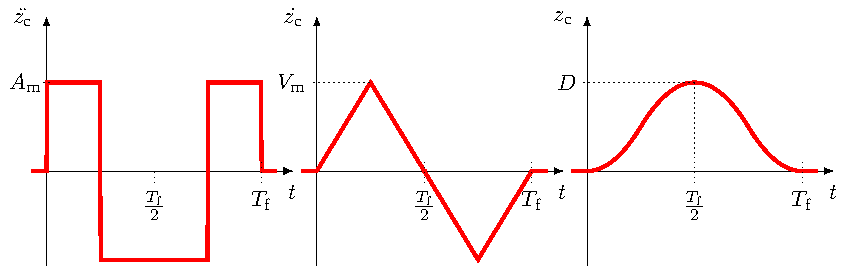
\includegraphics{P3/MonsterProfilAllerRetour}
\CaptionFigs{Représentation du \pacc utilisé pour nos expériences. Celui-ci correspond à un aller-retour, et est composé de phases d'accélération uniforme ($\AccZc$ et $-\AccZc$). Les vitesses~$\dzc$ et position~s$\zc$ correspondantes sont aussi représentées en fonction du temps $t$. Le mouvement durant un temps total $\tfin$, le piège s'éloigne de sa position d'origine de $\DistZc=\AccZc\,\ttfrac{\tfin^2}{16}$. La longueur totale parcourue est $2\,\DistZc=\AccZc\,\ttfrac{\tfin^2}{8}$}.
\label{fig:ProfilAllerRetour}
\efigh

Nous avons choisi d'effectuer un mouvement qui se décompose en quatre phases d'égale durée $\tfrac{\tfin}{4}$ et d'accélération uniforme, respectivement $\AccZc$, $-\AccZc$, $-\AccZc$, $\AccZc$.
La vitesse maximale $\VitZc$ %
\nome{\VitZc}{Valeur maximale de la vitesse du \pd}%
et la position maximale $\DistZc$ atteinte par le piège sont respectivement données par :
\[
\begin{cases}
	\VitZc  & = \AccZc\,\frac{\tfin}{4} \\
	~\DistZc & = \AccZc\,\frac{\tfin^2}{16} \\
\end{cases}
\pointformule
\]
 
\subsubsection{Mesure de l'amplitude $\Aosc$ des oscillations}
Afin de mesurer l'amplitude $\Aosc$ des oscillations après le transport, nous effectuons \val{30} prises d'images%
\footnote{Rappelons que, le processus d'imagerie étant destructif, chaque cliché correspond en fait à l'exécution d'une \seqexp. Seul l'instant de la prise d'image varie d'une séquence à l'autre.
}
 séparées de \ms{10} à partir du temps $t=\tfin$, correspondant à la fin du transport, \cad une fois que le \pd est arrêté en $z=0$.
La position $z(t>\tfin)$ du \cdm du \n est repérée en ajustant une fonction gaussienne \bde sur chaque image. 
Sur ces données de positions, nous ajustons alors une fonction sinusoïdale pour déduire l'amplitude $\Aosc$ des oscillations suivant l'axe longitudinal. 

\RemarqueTitre{Prédiction \sotosay{naïve}}{
%\inlinefig{%
%\begin{tikzpicture}[scale=1]
%\tkzInit[xmin=0,xmax=4,ymin=0,ymax=3]
%\tkzX[label=$\tfin$, orig, noticks, poslabel=-0.6cm]
%\tkzY[label=$\Aosc$, noticks, poslabel=-0.6cm]
%\tkzFct[samples = 100,color = red, lw=1.5pt](0.1..5){1/sqrt(\x)}
%\end{tikzpicture}
%}%
%\begin{minipage}{8.3cm}
En mesurant l'amplitude $\Aosc$ des oscillations après un transport sur une distance $\DistZc$ donnée, et dont la durée totale est $\tfin$, on pourrait \sotosay{naïvement} s'attendre à observer que :
\begin{itemize}
	\item plus la durée $\tfin$ est grande, plus le mouvement est lent, donc plus les oscillations en fin de transport auront une faible amplitude $\Aosc$.
	\item plus $\tfin$ est faible, plus le mouvement est violent, donc plus $\Aosc$ sera grand.
\end{itemize}
%\end{minipage}
}
\ifthenelse{\FormatEUE > 0}{}
{\RemonteUneLigne\AjouteLigne}

\subsubsection{Résultats}
La figure~\nref{fig:TransportDataAmplFit} représente, pour les \confab, la mesure de l'amplitude $\Aosc$ des oscillations après un transport en fonction de la durée totale $\tfin$ de ce transport. Le \pacc utilisé est celui représenté sur la figure~\nref{fig:ProfilAllerRetour}.
%
\bfighss
\subfloat[]{
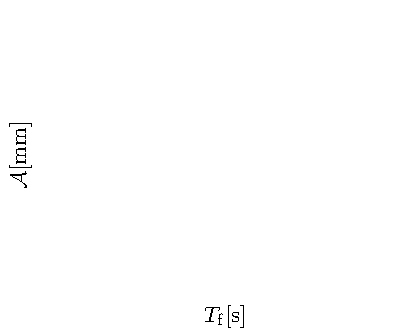
\includegraphics{P3/MonsterTransportDataAmplSchem1Fit}}
\subfloat[]{
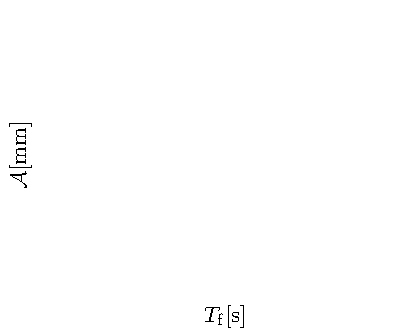
\includegraphics{P3/MonsterTransportDataAmplSchem2Fit}}
\CaptionFigs{Représentation, pour les \confab, de l'amplitude $\Aosc$ des oscillations après un transport en fonction de la durée totale $\tfin$ de ce transport. Le \pacc utilisé est celui représenté sur la figure~\nref{fig:ProfilAllerRetour}. On s'attend bien à observer une diminution de l'amplitude $\Aosc$ quand le temps de transport $\tfin$ augmente. On observe cependant une série de temps $\tfin$ pour lesquels $\Aosc$ est très faible.
La ligne continue rouge correspond à l'expression  théorique~\nref{eq:AoscProfilAllerRetour} déduite d'une modélisation par un \pphar \ud (voir la \autoref{sec:ModelisationTransport}). Pour la \confa, l'expression théorique a été ajustée grâce à un facteur multiplicatif globale~($\times\val{0.5}$).}
\label{fig:TransportDataAmplFit}
\efigh

On constate sur les données expérimentales, qu'il existe une série de temps $\tfin$ pour lesquels l'amplitude $\Aosc$ devient très faible.
Afin d'interpréter ces données, nous avons effectué une modélisation du transport qui fait l'objet de la \autoref{sec:ModelisationTransport}. Celle-ci rappelle des travaux initialement effectués pour décrire le transport d'ions piégés~\cite{RLB06}. L'expression obtenue pour l'amplitude en fin de transport est représentée sur la figure~\nref{fig:TransportDataAmplFit} (ligne continue rouge) et rend bien compte de l'existence de durées \emph{optimales} pour la mise en mouvement du \pd.

Sur nos expériences de transport, nous sommes actuellement limités par la vitesse et l'accélération maximales que nous autorise notre platine de translation%
\footnotemark.
Ceci limite les possibilités d'effectuer des transports en des temps courts, proches de la période d'oscillation propre du \pd. Sur les données expérimentales de la figure~\nref{fig:TransportDataAmplFit} les temps de transport minimaux sont d'environ $2$ périodes. %
%
\footnotetext{L'accélération maximale est d'environ \mpsc{5} et la vitesse maximale est d'environ \cmps{35}.}

\casse

\section{Modélisation pour un piège unidimensionnel harmonique}\label{sec:ModelisationTransport}

Pour étudier le problème de l'excitation d'un \n après un transport non-adiabatique, nous avons effectué une modélisation \ude en considérant un \pphar $\Uh(z,t)$, mobile suivant l'axe horizontal $z$ du déplacement:
\begin{equation}
	\Uh(z,t) = \frac{1}{2}\, m \,\PulsUh^2 \, (z-\zct)^2
	\pointformule
	\label{eq:Uh1D}
\end{equation}
où $\zct$ désigne la position du piège sur l'axe $z$ à chaque instant $t$. 

\subsection{Étude du mouvement du \cdm dans le référentiel du piège}

Dans la suite, nous considérons qu'à l'instant $t=0$ le \cdm du \nat est immobile au fond du piège, en $z=0$. 
\Resultat{
Une propriété particulièrement intéressante du \pphar est que le mouvement du \cdm d'un système à $N$ particules est complètement découplé des autres degrés de liberté et est \emph{indépendant de la nature des interactions} entre particules. Ce mode d'oscillation du \cdm est appelé \termetech{mode de Kohn}\footnotemark.

Dans toute la suite, nous étudierons le mouvement du \cdm du \n. Celui-ci sera traité comme le mouvement d'une seule particule dans le \pphar.
}
%
\footnotetext{Cette propriété remarquable a été étudiée pour des systèmes quantiques piégés par Kohn (1961) puis Brey \etal (1989)~\cite{Koh61,BJH89}.}%

Nous nous proposons d'étudier l'énergie mécanique communiquée au \nat
% dans le référentiel du piège,
 à la fin du mouvement (\ie en $t=\tfin$).
Afin de simplifier notre étude tout en conservant toute la généralité du problème, il est commode de se placer dans le référentiel du piège. Celui-ci n'est pas galiléen puisqu'il est animé d'une vitesse $\zct$ par rapport au \reflab. Il faut donc tenir compte du champ de forces d'inertie d'entrainement:
\begin{equation}
	\Fe(t) = -m\,\ddzct
	\label{eq:ForceInertie}
\end{equation}
%
\Remarque{Précisons que les forces d'inertie d'entrainement correspondent à un champ de force \emph{uniforme}. Ceci implique que dans le référentiel lié au piège, le \pp conserve sa forme harmonique. L'étude des \termetech{modes de Kohn} y reste donc valable%\footnotemark%
.}%
%\footnotetext{Il en aurait été autrement s'il avait fallu tenir compte, par exemple, de forces centrifuges, ou de forces de Coriolis.}
%

\casse


\subsection{Mouvement du \cdm du \n}
L'équation du mouvement du \cdm du \n, dont la position est notée $\zpt$ dans le référentiel du piège, s'obtient alors très simplement de manière formelle:
\begin{align}
	\zpt &= \frac{1}{m\,\PulsUh} \, 
	\IntegraleBornes{\Fe(u) \, \sin\bigl(\PulsUh\,(t-u)\bigr)}
	{\ddint u}{0}{t}
%	\nonumber \\ 	&
	= 	-\frac{1}{\PulsUh} \, \IntegraleBornes{\ddzc(u) \, \sin\bigl(\PulsUh\,(t-u)\bigr)}
	{\ddint u}{0}{t}
%	\nonumber \\
%	&= 	-\IntegraleBornes{\dzc(u) \, \cos\bigl(\PulsUh\,(t-u)\bigr)}
%	{\ddint u}{0}{t}
	\virguleformule
	\label{eq:MouvZp}
\end{align}
où nous avons tenu compte des conditions initiales~\nref{eq:ZcDzcIni}, et où la deuxième égalité est obtenue grâce à l'équation~\nref{eq:ForceInertie}. 
La vitesse $\vpt$ s'obtient en dérivant l'expression~\nref{eq:MouvZp}:
\begin{equation}
	\vpt % \equiv \Derive{\zpt}{t}	
%	= 	\IntegraleBornes{\PulsUh\,\dzc(u) \, \sin\bigl(\PulsUh\,(t-u)\bigr)}
%	{\ddint u}{0}{t} ~~ - ~~ \dzct
	= 	- \IntegraleBornes{\ddzc(u) \, \cos\bigl(\PulsUh\,(t-u)\bigr)}
	{\ddint u}{0}{t}
	\pointformule
	\label{eq:MouvVp}
\end{equation}



\subsection{Amplitude des oscillations en fin de transport}\label{sec:AmplFinTransport}

Nous sommes intéressés par l'amplitude $\Aosc$ des oscillations du \cdm du \n à la fin du transport. Celle-ci dépend de la position $\zp$ et de la vitesse $\vp$ dans le référentiel du piège au temps $t=\tfin$. 
\`A partir des équations~\nref{eq:MouvZp} et~\nref{eq:MouvVp}, on peut alors calculer l'amplitude $\Aosc$ en fin de transport par :
\begin{equation}
	\Aosc^2 = \zp(\tfin)^2 + \dfrac{\vp(\tfin)^2}{\PulsUh^2}
	\pointformule
	\label{eq:AoscZpVp}
\end{equation}

\noindent On peut exprimer $\Aosc$ d'une manière élégante si on remarque que les équations~\nref{eq:MouvZp} et~\nref{eq:MouvVp} peuvent être formulées comme suit:
\begin{equation}
	\begin{cases}
	~~~\zpt &= ~~ 
	\Reelle{ \frac{\im}{\PulsUh} \, \Expo{\im\,\PulsUh\,t} \, \IntegraleBornes{\ddzc(u) \, \Expo{-\im\,\PulsUh\,u}}
	{\ddint u}{0}{t} }
 \vspace{1ex}	\\
	-\frac{\vpt}{\PulsUh} &= ~~ 
	\Imaginaire{ \frac{\im}{\PulsUh} \, \Expo{\im\,\PulsUh\,t} \, \IntegraleBornes{\ddzc(u) \, \Expo{-\im\,\PulsUh\,u}}
	{\ddint u}{0}{t} }
	\end{cases}
	\virguleformule
	\label{eq:MouvZpVpExpo}
\end{equation}
où $\Reelle{}$ et $\Imaginaire{}$ désignent respectivement les parties réelle et imaginaire d'un nombre complexe. L'équation~\nref{eq:AoscZpVp} s'écrit alors sous la forme:
\[
	\Aosc^2 
	= \Module{
	\frac{\im}{\PulsUh} \, \Expo{\im\,\PulsUh\,t} \, \IntegraleBornes{\ddzc(u) \, \Expo{-\im\,\PulsUh\,u}}
	{\ddint u}{0}{\tfin}
	}^2 
	~~~ = ~~ ~~ \Module{
	\frac{\im}{\PulsUh} \, \Expo{\im\,\PulsUh\,t} \, \IntegraleBornes{\ddzc(u) \, \Expo{-\im\,\PulsUh\,u}}
	{\ddint u}{-\infty}{\infty}
	}^2 
	\virguleformule
%	\nonumber
%	\label{eq:AoscPrelim}
\]
où la deuxième égalité fait intervenir le fait que la fonction $\ddzc$ est nulle en dehors de l'intervalle~$\left[ \,0\, ;\, \tfin \,\right]$.
%
\Resultat{
On peut donc écrire une relation entre l'amplitude $\Aosc$ en fin de transport et le \pacc $\ddzct$:
\begin{equation}
	\Aosc = \frac{1}{\PulsUh} \, \Module{
	\Fourier{\ddzc}(\PulsUh)
	}
	\virguleformule
	\label{eq:AoscModuleFourier}
\end{equation}
où $\Fourier{g}(\PulsUh)$ désigne la \tf :
$\IntegraleBornes{g(u)\,\Expo{-\im\,\PulsUh\,u}}{\ddint u}{-\infty}{\infty}$\pointformule
}
%
Notons que dans l'expression~\nref{eq:AoscModuleFourier} la durée de transport $\tfin$ intervient implicitement dans la fonction $\ddzct$. Afin de la faire apparaître explicitement, nous proposons de définir un \pacc \termetech{normalisé}, $\ddzcnv$ %
\nome{\ddzcn}{Profil d'accélération \termetech{normalisé}}%
tel que:
\begin{equation}
%	\ddzct \equiv \AccZc\, \ddzcn\left(\frac{t}{\tfin}\right) 
	\ddzcnv \equiv \frac{\ddzc\left(\tadim\,\tfin\right)}{\AccZc}
	\virguleformule
	\label{eq:ddzcnormalise}
\end{equation}
où $\tfin$ est la durée du mouvement et $\AccZc$ est la valeur maximale de l'accélération en valeur absolue ($\AccZc>0$). 
\inlinefig{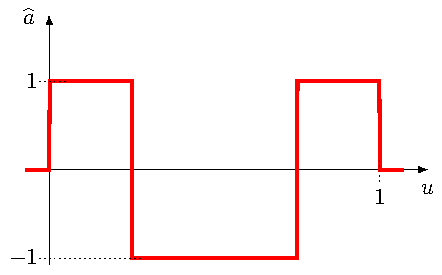
\includegraphics{P3/MonsterProfilNormaliseAllerRetour}~} 
\noindent Le \paccn ne prend des valeurs non-nulles que sur l'intervalle $[0;1]$ et ses valeurs sont comprises entre $-1$ et $1$.
Le \paccn décrit donc la \emph{forme} de la fonction $\ddzct$. Par exemple, le profil de la figure \vref{fig:ProfilAllerRetour}, qui correspond à un aller-retour, est entièrement décrit par la donnée du \pn $\ddzcnv$ (représentée ci-contre), de $\tfin$ et de la valeur maximale $\AccZc$ de l'accélération.
\picskip{0}
%
\Resultat{
Par un changement de variable, on peut donc ré-écrire l'expression~\nref{eq:AoscModuleFourier} en une équation faisant intervenir la forme $\ddzcn$ du profil, sa durée $\tfin$ et son amplitude $\AccZc$:
\begin{equation}
	\Aosc = \frac{\AccZc\,\tfin}{\PulsUh} \, \Module{
	\Fourier{\ddzcn}(\PulsUh\,\tfin)
	}
	= \AccZc\,\tfin^2 
	\times \frac{
	\Module{	\Fourier{\ddzcn}(\PulsUh\,\tfin)	}
	}{\PulsUh\,\tfin}
	\virguleformule
	\label{eq:AoscModuleFourierNormalise}
\end{equation}
où la deuxième égalité fait apparaître le terme $\AccZc\,\tfin^2$ qui est proportionnel à la distance totale parcourue (pour un \paccn donné). 
%Autrement dit, pour une distance de parcouru $\DistZc$ donnée, on pourra représenter 
}
%\Remarque{
%a
%}

\subsection{Confrontation aux données expérimentales; mélange non-linéaire}\label{sec:MelangeNonLineaire}
En appliquant la relation~\nref{eq:AoscModuleFourier} au \pacc utilisé expérimentalement pour faire faire un mouvement aller-retour au piège (voir la figure~\vref{fig:ProfilAllerRetour}), on obtient:
\begin{equation}
	\Aosc = 2\,\DistZc
	\,\sin_c^{\,2}\left(\frac{\PulsLong\,\tfin}{8}\right)
	\,\Module{\sin\left(\frac{\PulsLong\,\tfin}{4}\right)}
	\virguleformule
	\label{eq:AoscProfilAllerRetour}
\end{equation}
où $2\,\DistZc = \AccZc\,\ttfrac{\tfin^2}{8}$ est la distance totale parcourue durant le transport, et $\sin_c(u)$ désigne le sinus cardinal $\ttfrac{\sin(u)}{u}$.
Notons que la figure~\vref{fig:TransportDataAmplFit} montre que cette expression, appliquée aux cas des \confab, présente un très bon accord avec nos données expérimentales.  


\casse

\subsubsection{Atténuation des oscillations du \cdm par mélange non-linéaire}

Il faut noter sur la figure~\ref{fig:TransportDataAmplFit}, que pour la \confa, l'expression~\nref{eq:AoscProfilAllerRetour} a été ajustée par un facteur multiplicatif global~($\times\val{0.5}$). Ceci indique que pour cette configuration, les oscillations en fin de transport sont plus faibles que celles prédites par le modèle. 
%Il faut en effet garder à l'esprit que l

En réalité, ceci est dû au fait que le \n explore, durant le transport, une large plage du \pp. Celui-ci n'étant pas parfaitement harmonique, mais lorentzien, la pulsation $\PulsLongLor$ d'oscillation de chaque atome dépend en fait de l'amplitude de celle-ci (voir l'équation \vref{eq:PulsLongLor}).

La figure~\nref{fig:MonsterOscillPasMemePulsation} illustre le fait que l'extension spatiale du \n joue alors un rôle important. En effet, plus elle est grande, plus le \termetech{spectre} de pulsations du \n sera large. 
%Il en résulte un effet de brouillage sur la position du \cdm du nuage. 
Cet effet, qui provient des non-linéarités du \pp, est appelé \termetech{mélange non-linéaire} et induit un \emph{amortissement des oscillations du \cdm} du \n.
%
\bfighs
\subfloat[]{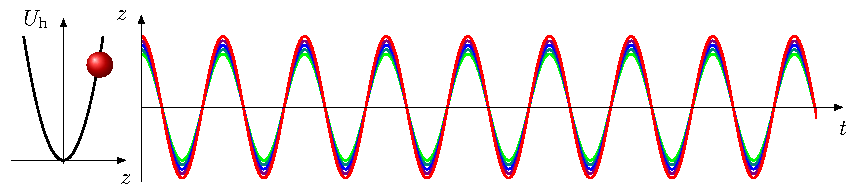
\includegraphics{P3/MonsterOscillTousMemePulsation}}\\
\RemonteUnPeuFig
\RemonteUnPeuFig
\RemonteUnPeuFig
\subfloat[]{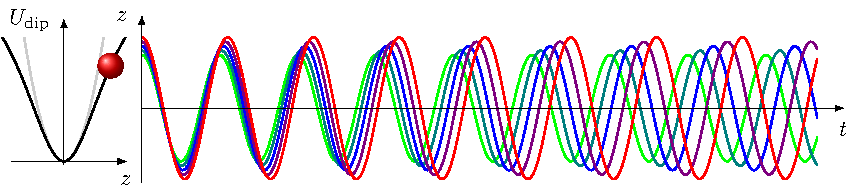
\includegraphics{P3/MonsterOscillPasMemePulsation}}\\
\RemonteUnPeuFig
\RemonteUnPeuFig
\RemonteUnPeuFig
\subfloat[]{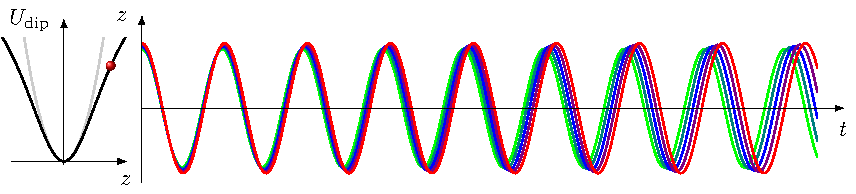
\includegraphics{P3/MonsterOscillPasMemePulsationPetitNuage}}\\
\CaptionFigs{Illustration schématique du \termetech{mélange non-linéaire}. Sur la gauche, un nuage est représenté dans le \pp. Les graphes sur la droite représentent quelques trajectoires atomiques du \n. Trois cas sont considérés :
\\
(a), dans un \pphar, tous les atomes ont la même pulsation d'oscillation. En conséquence, quelle que soit la taille du \n, on n'observe pas d'atténuation des oscillations du \cdm.
\\
(b), dans un \pp non-harmonique, la pulsation d'oscillation dépend de l'amplitude du mouvement de chaque atome. Ici, nous avons considéré la dépendance de l'expression~\nref{eq:PulsLongLor}. On observe alors un brouillage des oscillations du \cdm.
\\
(c), si la taille du \n est faible, le brouillage s'établit plus lentement puisque le spectre de pulsation représenté par le \n est plus étroit.}
\label{fig:MonsterOscillPasMemePulsation}
\efigh


\casse

\subsection{Analogie avec l'optique et l'analyse spectrale}
L'expression~\nref{eq:AoscModuleFourier}, qui permet de calculer l'amplitude $\Aosc$ des oscillations en fin de transport, est une simple \tf du \pacc. Sur le plan formel, il peut être intéressant de rapprocher cette expression de celle utilisée en optique pour décrire la diffraction de Fraunhofer%
\footnote{L'amplitude du champ électromagnétique diffracté dans une direction donnée est proportionnelle à la \tf de la transmittance de l'objet diffractant}%
~\cite{Goo05}, et en traitement du signal par analyse spectrale de Fourier~\cite{Har78}.
%
Cette analogie formelle peut grandement enrichir notre analyse dans la mesure où nous pouvons comparer :
\begin{itemize}
	\item la minimisation des oscillations consécutives à une mise en mouvement du piège,
	\item l'\termetech{apodisation} des faisceaux diffractés par une ouverture finie en optique,
	\item l'analyse de Fourier de signaux limités dans le temps qui fait intervenir des \termetech{fonctions de fenêtrage}.
\end{itemize}
Ces deux derniers problèmes ont en effet été largement étudiés et nous pouvons bénéficier des résultats obtenus dans ces domaine.

\ifthenelse{\FormatEUE > 0}{}
{\AjouteLigne}
%\AjouteLigne
%\AjouteLigne
\RemonteUnPeuFig
\RemonteUnPeuFig


\subsubsection{Exemple : le \pBH}
Un exemple de profil optimisé en analyse spectrale est le \pBH%
\footnote{Le \pBH est une fonction fenêtre définie sur l'intervalle $[0;1]$ par :\\$f(u)=\val{0.35875}-\val{0.48829}\,\cos(2\,\pi\,u)
+\val{0.14128}\,\cos(4\,\pi\,u)-\val{0.01168}\,\cos(6\,\pi\,u).
$}
\cite{Har78}. 
Ce profil est remarquable du fait que sa \tf est quasiment nulle%
\footnote{La \tf du \pBH est inférieure à \val{E-5} au delà de l'intervalle $[-4\,\pi ; 4\,\pi]$. Elle est d'ailleurs déjà inférieure à \val{E-2} au delà de l'intervalle $[-3\,\pi ; 3\,\pi]$.}
 en dehors de l'intervalle $[-4\,\pi ; 4\,\pi]$. 
Ceci signifie que les oscillations résiduelles seront très faibles, quel que soit le temps de transport $\tfin$, du moment que $\tfin$ est supérieur à \val{4} périodes d'oscillations (voir la figure~\nref{fig:MonsterProfilDeplacementHB}).
\bfighs
\subfloat{
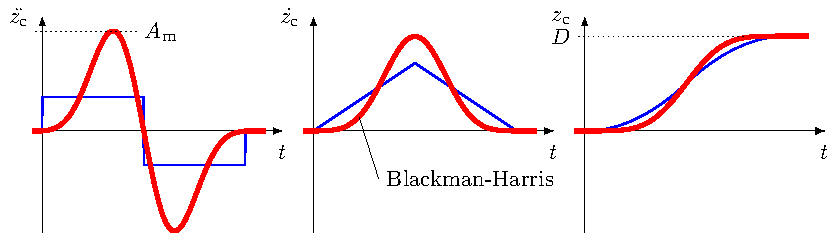
\includegraphics{P3/MonsterProfilDeplacementHB}}\\
\RemonteUnPeuFig
\RemonteUnPeuFig
\RemonteUnPeuFig
\subfloat{
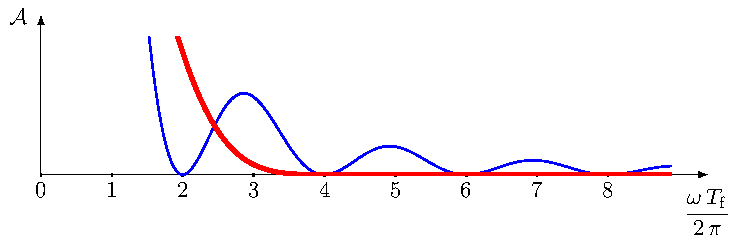
\includegraphics{P3/MonsterDeplacementHBAosc}}
\CaptionFigss{Représentation d'un \pacc correspondant à un déplacement d'une distance $\DistZc$ et faisant intervenir une fonction de \BH (trait rouge épais). Notons que c'est ici la vitesse $\dzc$ qui suit ce profil et l'accélération $\ddzc$ est calculée en dérivant $\dzc$. Le profil en trait fin bleu représente un mouvement de même déplacement $\DistZc$, mais fait de portions d'accélérations uniformes.
Le graphe inférieur représente (en unités arbitraires) l'amplitude des oscillations en fin de transport. Avec le \pBH, on constate l'absence quasi-totale d'oscillations dans le cas où le transport dure plus de $4$ périodes.}
\label{fig:MonsterProfilDeplacementHB}
\efigh

%\casse

Ce type de \pacc serait particulièrement adapté dans le cas où tous les atomes n'ont pas la même période d'oscillations propres, comme par exemple:
\begin{itemize}
	\item quand le potentiel \sotosay{vu} par les atomes dépend de leur état interne,	
	\item dans un piège contenant deux espèces atomiques.
\end{itemize}
Il suffit alors d'effectuer le mouvement en un temps quatre fois supérieur à la plus grande des périodes d'oscillations propres.


\subsection{Transport sur des durées inférieures à la période d'oscillation propre}
Nous avons montré qu'il est possible d'effectuer un déplacement non-adiabatique, sans induire d'oscillations du \cdm du \n après cette opération. Cependant, les données expérimentales ainsi que les exemples présentés dans ce chapitre, ne concerne que des temps de transport $\tfin$ supérieurs à la période d'oscillation propre du piège.
Pour finir cette section, nous donnons un exemple théorique de \pacc qui permet de déplacer un \n en un temps arbitrairement faible. 
Ce profil, représenté sur la figure~\nref{fig:TransportUltraRapide}, n'est bien sûr qu'un exemple (assez simple), faisant intervenir des phases d'accélérations uniformes.
%
\bfighs
\subfloat{
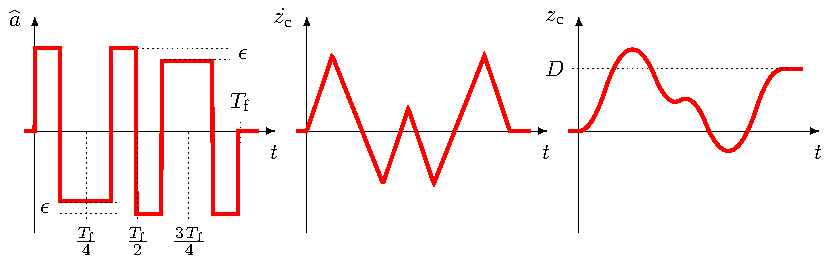
\includegraphics{P3/MonsterTransportUltraRapide}}\\
\RemonteUnPeuFig
\RemonteUnPeuFig
\subfloat{
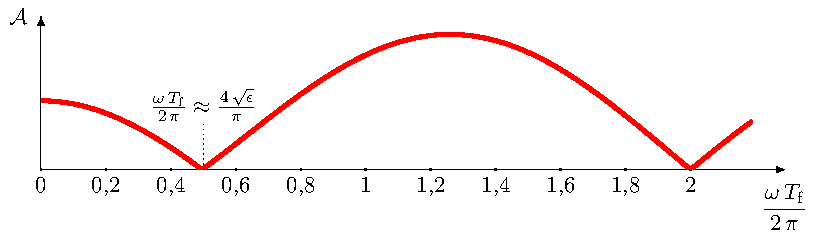
\includegraphics{P3/MonsterTransportUltraRapideAosc}}
\CaptionFigs{Représentation d'un \pacc permettant d'effectuer le transport en un temps $\tfin$ arbitrairement faible. Plus le paramètre $\epsilon$ est faible, plus le temps de transport pourra être bref, mais plus le déplacement $\DistZc$ sera faible. Le graphe inférieur représente (en unités arbitraires) l'amplitude des oscillations en fin de transport (nous avons choisi $\epsilon=0.15$).}
\label{fig:TransportUltraRapide}
\efigh


Il faut bien sûr garder à l'esprit que, pour une distance de transport $\DistZc$ donnée, plus le temps $\tfin$ est bref, plus le mouvement du \pd sera violent. En pratique, deux facteurs limites le transport sur des échelles de temps inférieures à la période d'oscillation:
\begin{itemize}
	\item les limites de vitesse et d'accélération du piège,
	\item la raideur et la profondeur du \pc selon la direction du mouvement.
\end{itemize}


\casse


\subsection{Conclusion}% et perspectives}

Nous avons montré dans ce chapitre que le \fld semble être une bonne manière de produire, puis de mettre en mouvement des \patufs et denses. 
Les résultats présentés dans la section précédente montrent qu'il est possible de mettre rapidement en mouvement un \nat piégé de manière \termetech{optimale}, \cad sans affecter ces caractéristiques après le mouvement.

La perspective ouverte par ces résultats est celle d'un \setup combinant le \fld et un \gm. On pourrait alors injecter des \pats denses avec un bon taux de répétition. Les \paccs qui ont été présenté dans ce chapitre (figure~\nref{fig:ProfilAllerRetour} et~\nref{fig:ProfilDeplacement}), correspondent à des \sotosay{déplacements} du \pd, \cad à un mouvement dont l'état final possède une vitesse nulle. On peut cependant considérer des \paccs se terminant par une vitesse finie du piège (voir la figure~\nref{fig:MonsterProfilLancementHB}).
%
\bfighs
\subfloat{
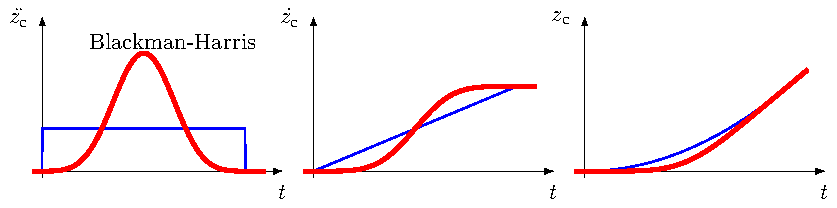
\includegraphics{P3/MonsterProfilLancementHB}}\\
\RemonteUnPeuFig
\RemonteUnPeuFig
\RemonteUnPeuFig
\RemonteUnPeuFig
\subfloat{
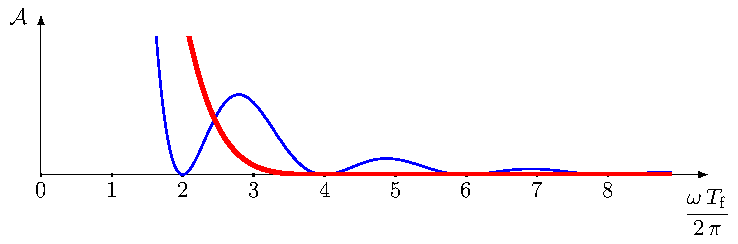
\includegraphics{P3/MonsterLancementAosc}}
\CaptionFigs{Représentation d'un \pacc correspondant à un \sotosay{lancement}. Le profil en trait fin bleu représente un mouvement d'accélération uniforme conduisant à la même vitesse finale.
L'amplitude des oscillations dans le référentiel en mouvement à la fin du lancement est représentée sur le graphe inférieur représente (en unités arbitraires).}
\label{fig:MonsterProfilLancementHB}
\efigh



%\subsection{Compression par zoom optique}\label{sec:ZoomOptique}
%
%
%Dans la \autoref{sec:Proportionalite}, nous avons donné quelques lois de proportionnalité pour les caractéristiques du \pd et d'un \nat qui y serait à l'\eqthdy. Il est important de remarquer que les trois grandeurs physiques :
%\begin{itemize}
%	\item la \dat moyenne $\overline{\dens}$,
%	\item la \dmdedpup $\overline{\rho}$, 
%	\item le \tcolel moyen par atome $\overline{\gammacol}$,
%\end{itemize}
%dépendent toutes de la valeur du \waist suivant une loi en $\ttfrac{1}{\wzero^7}$ (toute autre chose étant égale par ailleurs).
%
%compression~\cite{HDW01}
%compression \bec~\cite{KWW05}
%
%\subsection{Lancement du \nat}\label{sec:LancementNat}
%



